\documentclass[5p,times]{elsarticle}

% Math and symbols
\usepackage{amsmath,amssymb,amsfonts}
\usepackage{bm}

% Figures and tables
\usepackage{graphicx}
\usepackage{booktabs}
\usepackage{multirow}
\usepackage{subfig}
\usepackage{array}
\usepackage{tabularx}
\newcolumntype{C}{>{\centering\arraybackslash}X}
\usepackage{float}

% Colors and links
\usepackage{xcolor}
\usepackage{hyperref}
\hypersetup{
    colorlinks=true,
    linkcolor=blue,
    filecolor=magenta,
    urlcolor=cyan,
    citecolor=blue
}

% Algorithms
\usepackage{algorithm}
\usepackage{algorithmic}
\floatname{algorithm}{Algorithm}
\renewcommand{\algorithmicrequire}{\textbf{Input:}}
\renewcommand{\algorithmicensure}{\textbf{Output:}}

% Code
\usepackage{listings}

% Others
\usepackage{url}
\usepackage{enumitem}
\usepackage{threeparttable}

% Image path
\graphicspath{{figures/}}

\begin{document}

\begin{frontmatter}

\title{"Missing as Signal": MIM-Based SOH Prediction for Lithium-Ion Batteries Using Deep Learning}

\author[inst1]{Qingyang Chen}
\ead{202414544@mail.sdu.edu.cn}
\author[inst1]{Qiang Zhang\corref{cor1}}
\ead{sduzhangqiang@sdu.edu.cn}
\author[inst2]{Yunfei Wang}
\cortext[cor1]{Corresponding author.}

\address[inst1]{School of Nuclear Science and Energy Engineering, Shandong University, Jinan 250061, China}
\address[inst2]{Shandong Supermaly Generating Equipment Co., Ltd, No.5153 Yingqian Street, Hi-technology Development Zone, Weifang 261061, Shandong, China}

\begin{abstract}
Accurate State of Health (SOH) estimation is essential for safe and reliable operation of electric vehicles and energy storage systems, yet sensor failures and data acquisition anomalies frequently cause missing monitoring data. Traditional methods treat missing values as noise, neglecting the information contained in the pattern of missingness itself, which limits performance at high missing rates. Based on the public XJTU lithium-ion battery dataset, a Missing Indicator Matrix (MIM) approach is introduced and its impact on SOH prediction is systematically evaluated across four deep learning architectures---MLP, LSTM, GRU, and 1D-CNN---under varying missing-rate conditions. Results demonstrate that for missing rates $\geq$0.4, MIM consistently improves prediction accuracy, reducing error by 26--57\% across all models compared to imputation-only baselines. The improvement is observed uniformly across architectures, indicating that the missing-indicator signal is more valuable than the imputation method itself. This study provides a concise, effective technical solution for handling missing data in Battery Management Systems, enhancing the practicality and reliability of data-driven SOH prediction methods in real-world engineering applications.
\end{abstract}

\begin{keyword}
lithium-ion battery \sep State of Health (SOH) prediction \sep missing data \sep Missing Indicator Matrix (MIM) \sep XJTU dataset \sep deep learning
\end{keyword}

\end{frontmatter}

%==============================================================================
\section{Introduction}\label{sec:intro}

Against the backdrop of global energy structure transformation and rapid development of transportation electrification, lithium-ion batteries have been deployed at large scale in electric vehicles, grid-scale energy storage, and distributed energy systems. Accurate estimation and prediction of battery State of Health (SOH) is essential for ensuring system operational safety, optimizing energy management strategies, and controlling full lifecycle costs. In large-scale electric vehicle fleets and grid-scale energy storage systems, SOH estimation accuracy directly affects capacity planning and dispatch strategies, serving as an important foundation for ensuring high penetration of renewable energy sources.

In recent years, data-driven SOH prediction methods have received widespread attention\cite{luo2022review}. These methods learn complex nonlinear mapping relationships between features and SOH from historical operational data, avoiding the construction of complex electrochemical mechanism models, and demonstrating clear advantages in adaptability and scalability. Various algorithms, from shallow models to deep neural architectures\cite{liu2025deep,shao2023review,wang2023battery}, have continuously improved prediction accuracy on publicly available benchmark datasets, laying a solid foundation for the engineering application of SOH prediction.

However, in practical engineering scenarios, sensor data collected by Battery Management Systems (BMS) often suffers from varying degrees of missing data. The main causes include sensor failures and aging, unstable communication links causing data packet loss, and sampling strategy optimization or protection mechanism triggering leading to intermittent recording interruptions. In large-scale energy storage stations or fleet-level application scenarios, this problem is particularly prominent due to the large number of batteries and dense monitoring points.

When input features exhibit significant missing data, traditional data-driven models often face issues such as inconsistent input dimensions, feature distribution shifts, and increased prediction uncertainty. In current practice, these missing problems are often addressed through data screening or conservative strategies, resulting in substantial reduction of available samples and making SOH prediction models difficult to generalize to real-world complex operating conditions. Figure~\ref{fig:problem_scenario} illustrates the BMS monitoring chain and the cycle-level feature matrix with MCAR missing patterns.

\begin{figure*}[!htb]
    \centering
    
\includegraphics[width=\textwidth]{fig1_problem_scenario.png}
    \caption{Schematic diagram of data missing problems in battery SOH prediction. (a) BMS monitoring chain and potential failure sources; (b) Cycle-level feature matrix and MCAR missing patterns.}
    \label{fig:problem_scenario}
\end{figure*}

%------------------------------------------------------------------------------
\subsection{Literature Review}\label{sec:literature}

Battery SOH prediction has evolved from physics-based to data-driven modeling approaches. Early physics-based methods described internal battery aging mechanisms through electrochemical impedance spectroscopy and equivalent circuit models\cite{wang2020phys,yang2019ecm}, offering clear physical interpretability, but with numerous model parameters that are difficult to identify and poor adaptability to different chemistries and operating conditions. With the development of machine learning technology, data-driven methods have gradually become mainstream\cite{liu2025deep,shao2023review,wang2023battery}, which can be roughly divided into three categories: feedforward networks (MLP)\cite{bairwa2025cycle}, recurrent neural networks (LSTM/GRU)\cite{hochreiter1997lstm,cho2014gru}, and one-dimensional convolutional neural networks (1D-CNN)\cite{lecun2015cnn,zhang2024cnnsoh}.

Regarding missing data problems in BMS monitoring data, existing research adopts three categories of treatment strategies\cite{little2002statistical,rubin1976inference}: deletion methods discard samples or features containing missing values but cause severe information loss at high missing rates; imputation methods fill missing values through statistics or prediction models yet struggle to characterize uncertainty and cannot encode ``which features are missing where''\cite{jones1996indicator,van2023missing}; model-based methods require complex distribution assumptions with high computational costs, making deployment difficult in resource-constrained BMS environments. These traditional methods generally follow the ``repair data first, then predict'' paradigm, treating missing data as noise rather than potential signals. In contrast, the Missing Indicator Matrix (MIM) method provides an alternative approach by explicitly encoding missing patterns as additional binary features, feeding them into the model together with original features\cite{jones1996indicator,van2023missing}. This ``missing as signal'' paradigm has been successfully applied in medical data analysis, recommendation systems, and other domains\cite{sisk2023imputation,ehrig2025imputation,ipsen2022deal,che2018recurrent}, showing significant performance improvements when missing patterns are informative.

%------------------------------------------------------------------------------
\subsection{Research Gap and Contributions}\label{sec:contributions}

Despite the availability of rich datasets and advanced deep learning techniques, most existing SOH prediction research assumes that input data is essentially complete, with less systematic consideration of data missing problems\cite{shao2025soh,deng2025novel,chen2024batteryMissing}. This study identifies three key gaps in the current literature. First, existing SOH estimation work predominantly assumes data completeness, lacking systematic investigation into how various missing rates affect prediction performance in real-world BMS applications. Second, there is a lack of comprehensive evaluation frameworks that systematically assess MIM effectiveness across multiple missing rates and diverse deep learning architectures under strictly controlled experimental conditions. Third, current literature provides limited actionable guidance for BMS practitioners on selecting appropriate model architectures and MIM configurations based on specific missing rate intervals and hardware constraints.

To address these gaps, this paper proposes the ``missing as signal'' modeling paradigm and systematically evaluates the MIM method for battery SOH prediction. The core contributions include systematically proposing and validating the ``missing as signal'' paradigm in battery SOH prediction, shifting from the traditional ``impute first, then predict'' workflow to an end-to-end joint learning approach that treats missing patterns as first-order input features. This work constructs a unified evaluation benchmark covering nine levels of missing rates, four representative deep learning architectures, and rigorous statistical validation through 100 random seeds, providing comprehensive insights into MIM effectiveness across diverse scenarios. A multi-missing-rate joint training strategy is proposed that enables a single MIM model to maintain robust performance when facing unknown missing patterns, enhancing practical deployability in complex operating conditions. Finally, quantitative model selection recommendations mapping missing rate intervals to optimal architecture-MIM combinations are provided, offering actionable guidance for BMS design in electric vehicles and energy storage systems.

%------------------------------------------------------------------------------
\subsection{Paper Organization}\label{sec:organization}

The remainder of this paper is organized as follows. Section~\ref{sec:method} presents the proposed methodology, including problem formulation, MIM input construction, multi-missing-rate joint training strategy, and deep learning architectures. Section~\ref{sec:dataset} describes the XJTU battery dataset, feature engineering, missing simulation settings, and experimental setup. Section~\ref{sec:results} presents the experimental results, performance analysis, and statistical significance tests, followed by discussion of the MIM mechanism, architecture-wise analysis, and BMS-oriented configuration recommendations. Finally, Section~\ref{sec:conclusion} summarizes the findings and outlines future research directions.

%==============================================================================
\section{Methodology}\label{sec:method}

This section presents the proposed methodology for battery SOH prediction under missing data conditions. The technical framework encompasses problem formulation, MIM-based input construction, multi-missing-rate joint training strategy, and deep learning architectures.

%------------------------------------------------------------------------------
\subsection{Problem Formulation and Notation}\label{sec:formulation}

The SOH prediction task is formulated as a supervised regression problem. Let $\mathcal{D} = \{(\mathbf{x}_i, y_i)\}_{i=1}^{n}$ denote the dataset consisting of $n$ samples, where $\mathbf{x}_i \in \mathbb{R}^{d}$ represents the $d$-dimensional feature vector extracted from the $i$-th charge-discharge cycle, and $y_i \in [0, 1]$ denotes the corresponding SOH value defined as the ratio of current discharge capacity to initial rated capacity:
\begin{equation}
    y_i = \frac{Q_i}{Q_0}
    \label{eq:soh}
\end{equation}
where $Q_i$ is the measured discharge capacity of the $i$-th cycle and $Q_0$ is the initial rated capacity.

In practice, due to sensor failures and communication issues, the feature vector $\mathbf{x}_i$ may contain missing values. We define the observed feature vector as $\mathbf{x}_i^{\text{obs}}$ and introduce a binary missing indicator vector $\mathbf{m}_i \in \{0, 1\}^{d}$, where each element indicates whether the corresponding feature is missing:
\begin{equation}
    m_{ij} = 
    \begin{cases}
        0, & \text{if } x_{ij} \text{ is observed} \\
        1, & \text{if } x_{ij} \text{ is missing}
    \end{cases}
    \label{eq:indicator}
\end{equation}

The missing rate (MR) for the entire dataset is defined as the proportion of missing elements:
\begin{equation}
    \text{MR} = \frac{1}{n \cdot d} \sum_{i=1}^{n} \sum_{j=1}^{d} m_{ij}
    \label{eq:mr}
\end{equation}

To handle missing values, we employ mean imputation to obtain the imputed feature vector $\hat{\mathbf{x}}_i$, where missing values are replaced by the mean of the corresponding feature computed from observed values in the training set. The objective is to learn a prediction function $f: \mathcal{X} \rightarrow \mathcal{Y}$ that maps from the input space to SOH estimates, minimizing the expected prediction error.

%------------------------------------------------------------------------------
\subsection{MIM Input Construction}\label{sec:mim}

Traditional approaches to missing data in SOH prediction follow a two-stage ``impute first, then predict'' paradigm, where missing values are filled before model training, and the missing indicator information is discarded. This study adopts the ``missing as signal'' paradigm, explicitly encoding missing patterns as informative features to enhance prediction robustness.

\subsubsection{Missing Mechanism Assumption}

This work adopts the Missing Completely at Random (MCAR) assumption for constructing controlled missing data scenarios\cite{little2002statistical,rubin1976inference}. Under MCAR, the probability of missingness is independent of both observed and unobserved data values. While real-world missing patterns may exhibit more complex dependencies, MCAR provides a principled Baseline for evaluating method robustness and enables systematic performance assessment across varying missing rates.

\subsubsection{Input Representation Strategies}

Two input representation strategies are constructed for comparative analysis:

The Baseline approach uses only the imputed feature vector as input:
\begin{equation}
    \mathbf{z}_i^{\text{base}} = \hat{\mathbf{x}}_i \in \mathbb{R}^{d}
\end{equation}
where $\hat{\mathbf{x}}_i$ is obtained through mean imputation. In this representation, the information about which features were originally missing is completely lost.

The Missing Indicator Matrix (MIM) approach augments the imputed features with the binary missing indicator vector:
\begin{equation}
    \mathbf{z}_i^{\text{MIM}} = [\hat{\mathbf{x}}_i \,|\, \mathbf{m}_i] \in \mathbb{R}^{2d}
\end{equation}
where $[\cdot|\cdot]$ denotes vector concatenation. This extended representation explicitly encodes both the imputed feature values and the missing pattern, enabling the model to learn the joint effects of feature values and missing indicators on SOH prediction.

The MIM construction process is formalized in Algorithm~\ref{alg:mim}. Given a raw feature matrix and a target missing rate, the algorithm samples a missing mask according to the MCAR mechanism, constructs the missing indicator matrix, performs mean imputation, and concatenates the imputed features with missing indicators to form the extended input.

\begin{algorithm}[!htb]
\caption{MIM Input Construction}
\label{alg:mim}
\begin{algorithmic}[1]
\REQUIRE Raw feature matrix $X \in \mathbb{R}^{n \times d}$, missing rate $p \in [0, 1]$
\ENSURE Imputed features $\hat{X}$, missing indicators $M$, extended input $Z$
\STATE Sample missing mask: $\Omega_{ij} \sim \text{Bernoulli}(1-p)$
\STATE Construct indicator matrix: $M_{ij} = \mathbb{I}(\Omega_{ij} = 0)$
\STATE Compute feature means: $\bar{x}_j = \frac{1}{n_j^{\text{obs}}} \sum_{i: \Omega_{ij}=1} X_{ij}$
\STATE Impute missing values: $\hat{X}_{ij} = \begin{cases} X_{ij}, & \text{if } \Omega_{ij}=1 \\ \bar{x}_j, & \text{if } \Omega_{ij}=0 \end{cases}$
\STATE Concatenate: $Z = [\hat{X} \,|\, M]$
\STATE \textbf{return} $\hat{X}$, $M$, $Z$
\end{algorithmic}
\end{algorithm}

Figure~\ref{fig:baseline_vs_mim} illustrates the structural difference between the Baseline and MIM input strategies. The Baseline strategy discards missing pattern information, while MIM preserves this information as explicit binary features, allowing the model to potentially learn reliability weighting based on missing indicators.

\begin{figure}[!htb]
    \centering
    
\includegraphics[width=\columnwidth]{fig2_baseline_vs_mim.png}
    \caption{Comparison of Baseline and MIM input strategies. (a) Baseline: 16-dimensional imputed features $\hat{X}$; (b) MIM: concatenated 32-dimensional extended input $[\hat{X} \,|\, M]$.}
    \label{fig:baseline_vs_mim}
\end{figure}

%------------------------------------------------------------------------------
\subsection{Multi-Missing-Rate Joint Training Strategy}\label{sec:training}

A critical challenge in deploying SOH prediction models under missing data conditions is ensuring robustness across varying missing rates. This study proposes a multi-missing-rate joint training strategy that explicitly exposes the model to diverse missing patterns during training.

\subsubsection{Training Data Augmentation}

For MIM-enabled models, the training process incorporates multiple missing rates simultaneously. Let $\mathcal{P} = \{0.0, 0.05, 0.1, 0.15, \ldots, 0.95\}$ denote the set of missing rates used for training. For each missing rate $p \in \mathcal{P}$, a copy of the training set is generated with missing values injected according to the MCAR mechanism, and MIM inputs are constructed. These augmented datasets are merged into a unified training set:
\begin{equation}
    \mathcal{D}_{\text{train}}^{\text{aug}} = \bigcup_{p \in \mathcal{P}} \{(Z^{(p)}_i, y_i)\}_{i=1}^{n_{\text{train}}}
\end{equation}
where $Z^{(p)}_i$ represents the MIM input for sample $i$ with missing rate $p$.

\subsubsection{Training Strategy Comparison}

The training strategies for Baseline and MIM models differ fundamentally:

Baseline models are trained exclusively on complete data (MR = 0.0). Training on data with missing values without explicit missing indicators introduces noise that the model cannot distinguish from actual feature variation, potentially degrading performance.

MIM models are trained on the augmented dataset $\mathcal{D}_{\text{train}}^{\text{aug}}$ containing samples with varying missing rates. During each training iteration, mini-batches are sampled from this augmented set, exposing the model to diverse missing patterns. This enables the model to learn robust representations that generalize across different missing conditions.

The multi-missing-rate joint training process is formalized in Algorithm~\ref{alg:training}. The algorithm iterates over the missing rate set, generates MIM inputs for each rate, merges them into an augmented training set, and performs standard mini-batch training with early stopping.

\begin{algorithm}[!htb]
\caption{Multi-Missing-Rate Joint Training}
\label{alg:training}
\begin{algorithmic}[1]
\REQUIRE Training set features $X$, labels $Y$, missing rate set $\mathcal{P}$
\ENSURE Trained MIM model $f_{\text{MIM}}$
\STATE Initialize augmented set: $\mathcal{D}_{\text{aug}} \leftarrow \emptyset$
\FOR{$p \in \mathcal{P}$}
    \STATE Generate MIM inputs: $(\hat{X}^{(p)}, M^{(p)}, Z^{(p)}) \leftarrow \text{Algorithm~\ref{alg:mim}}(X, p)$
    \STATE Merge: $\mathcal{D}_{\text{aug}} \leftarrow \mathcal{D}_{\text{aug}} \cup \{(Z^{(p)}, Y)\}$
\ENDFOR
\STATE Initialize model parameters $\theta$
\FOR{epoch $= 1, 2, \ldots$}
    \STATE Sample mini-batch from $\mathcal{D}_{\text{aug}}$
    \STATE Compute loss and update $\theta$
    \STATE Evaluate on validation set
    \STATE \textbf{if} validation loss not improving \textbf{then} early stopping
\ENDFOR
\STATE \textbf{return} $f_{\text{MIM}}$
\end{algorithmic}
\end{algorithm}

Figure~\ref{fig:joint_training} illustrates the multi-missing-rate joint training process. By training on samples with diverse missing rates, the model learns to handle missing patterns as a core aspect of the prediction task rather than treating them as noise to be ignored.

\begin{figure*}[!htb]
    \centering
    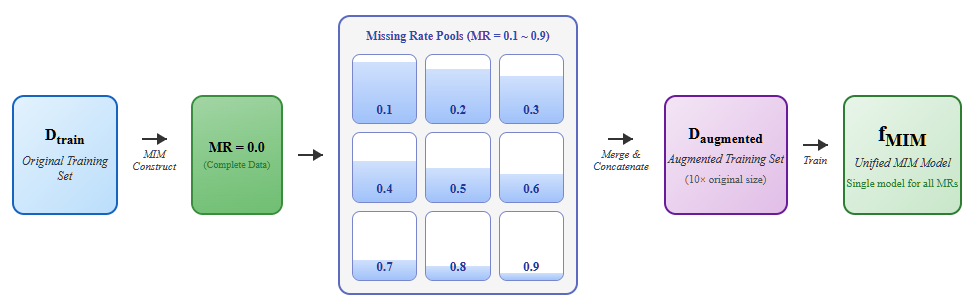
\includegraphics[width=\textwidth]{fig4_joint_training.png}
    \caption{Multi-missing-rate joint training process. The original training set generates copies at 20 missing rates (step 0.05), which after MIM construction are merged into $\mathcal{D}_{\text{augmented}}$ for training a unified MIM model.}
    \label{fig:joint_training}
\end{figure*}

%------------------------------------------------------------------------------
\subsection{Deep Learning Architectures}\label{sec:architectures}

To comprehensively evaluate the effectiveness of the MIM approach across different model families, four representative deep learning architectures are adopted: Multilayer Perceptron (MLP), Long Short-Term Memory (LSTM), Gated Recurrent Unit (GRU), and One-Dimensional Convolutional Neural Network (1D-CNN). These architectures span three distinct inductive biases: feedforward mapping, sequential modeling, and local pattern extraction.

\subsubsection{MLP: Feedforward Baseline}

The Multilayer Perceptron serves as the fundamental Baseline, learning direct mappings from input features to SOH without explicit sequential or spatial assumptions. The architecture consists of four fully-connected hidden layers with dimensions progressively reducing from input to output:
\begin{equation}
    d_{\text{input}} \rightarrow 192 \rightarrow 96 \rightarrow 48 \rightarrow 24 \rightarrow 1
\end{equation}
Each hidden layer applies ReLU activation, followed by dropout with rate 0.15 for regularization. The MLP establishes a performance Baseline that more sophisticated architectures should improve upon.

\subsubsection{LSTM: Sequential Modeling}

Long Short-Term Memory networks explicitly model temporal dependencies in battery cycling data through gated recurrent units. The architecture employs a two-layer LSTM with 48 hidden units per layer, processing sequences of length 5 cycles. Dropout with rate 0.2 is applied between layers to prevent overfitting. The LSTM's gating mechanisms enable selective retention of relevant historical information, potentially capturing aging trends and capacity regeneration patterns.

\subsubsection{GRU: Gated Recurrent Alternative}

Gated Recurrent Units offer a streamlined alternative to LSTM with fewer parameters while maintaining similar sequential modeling capabilities. The architecture uses a two-layer GRU with 64 hidden units per layer and sequence length 5, with dropout rate 0.2. GRU's simplified gating structure (reset and update gates only) may offer computational advantages while preserving the ability to model cycle-to-cycle dependencies.

\subsubsection{1D-CNN: Local Pattern Extraction}

One-Dimensional Convolutional Neural Networks extract local feature patterns along the temporal dimension through sliding convolutional filters. The architecture comprises two convolutional layers with channel dimensions $16 \rightarrow 72 \rightarrow 32$, kernel size 4, followed by adaptive pooling and fully-connected layers. Dropout with rate 0.1 is applied. The 1D-CNN's local receptive fields and weight sharing enable efficient parallel computation and may capture localized aging signatures.

\subsubsection{Model Configuration Summary}

Table~\ref{tab:model_config} summarizes the architectural configurations and parameter counts for all four models under both Baseline and MIM input strategies. Parameter counts are controlled within the range of 15k--45k to ensure fair comparison focused on input representation rather than model capacity. When switching from Baseline ($d$-dimensional input) to MIM ($2d$-dimensional input), parameter counts increase proportionally due to the expanded first-layer weight matrices.

\begin{table*}[!htbp]
\centering
\small
\caption{Deep Learning Architecture Configurations}
\label{tab:model_config}
\begin{tabularx}{\textwidth}{@{}llXrr@{}}
\toprule
\textbf{Model} & \textbf{Architecture} & \textbf{Key Hyperparameters} & \textbf{Baseline Params} & \textbf{MIM Params} \\
\midrule
MLP & FC$(d \rightarrow 192 \rightarrow 96 \rightarrow 48 \rightarrow 24 \rightarrow 1)$ & ReLU, Dropout=0.15 & 27,649 & 36,865 \\
LSTM & 2-layer LSTM + FC & hidden=48, seq=5, Dropout=0.2 & 31,537 & 40,753 \\
GRU & 2-layer GRU + FC & hidden=64, seq=5, Dropout=0.2 & 40,769 & 49,985 \\
1D-CNN & Conv1d$(d \rightarrow 72 \rightarrow 32)$ + FC & kernel=4, Dropout=0.1 & 16,713 & 30,537 \\
\bottomrule
\end{tabularx}
\end{table*}

Figure~\ref{fig:model_architectures} visualizes the structural designs of the four architectures, highlighting their distinct approaches to processing battery cycle features.

\begin{figure*}[!htb]
    \centering
    
\includegraphics[width=0.85\textwidth]{fig3_model_architectures.png}
    \caption{Comparison of four deep learning model architectures. (a) MLP; (b) LSTM; (c) GRU; (d) 1D-CNN.}
    \label{fig:model_architectures}
\end{figure*}

%------------------------------------------------------------------------------
\subsection{Loss Function and Optimization}\label{sec:optimization}

\subsubsection{Loss Function}

The SOH prediction task is formulated as a regression problem. The Mean Squared Error (MSE) loss is employed to measure the discrepancy between predicted and actual SOH values:
\begin{equation}
    \mathcal{L}(\theta) = \frac{1}{n} \sum_{i=1}^{n} \left( f_{\theta}(\mathbf{z}_i) - y_i \right)^2
\end{equation}
where $f_{\theta}$ denotes the neural network with parameters $\theta$, $\mathbf{z}_i$ represents the input (either Baseline or MIM), and $y_i$ is the true SOH label. MSE is chosen for its differentiability and sensitivity to large errors, appropriate for regression tasks where prediction accuracy is critical.

\subsubsection{Optimization}

Model parameters are optimized using the Adam algorithm, an adaptive first-order optimization method that maintains separate learning rates for each parameter based on estimates of first and second moments of gradients. The optimization process minimizes the MSE loss over the training data.

\subsubsection{Training Procedure}

The training procedure incorporates several regularization and convergence monitoring techniques:

Training is halted when validation loss ceases to improve for a specified number of consecutive epochs (patience). This prevents overfitting and ensures model generalization.

Dropout is applied at specified rates after hidden layers (see Table~\ref{tab:model_config}), randomly deactivating neurons during training to prevent co-adaptation.

Z-score normalization is applied to input features as a preprocessing step (detailed in Section~\ref{sec:dataset}), rather than using batch normalization.

The specific hyperparameter values and training configurations are documented in Section~\ref{sec:dataset}, which provides the complete experimental setup including learning rates, batch sizes, and hardware environment.

%==============================================================================
\section{Dataset and Experimental Setup}\label{sec:dataset}

This section describes the implementation environment, data preprocessing pipeline, missing data generation protocol, evaluation methodology, and experimental setup. All experiments are conducted on the publicly available XJTU battery aging dataset under strictly controlled conditions to ensure reproducibility and fair comparison.

%------------------------------------------------------------------------------
\subsection{XJTU Battery Dataset}\label{sec:xjtu}

The experiments utilize the XJTU lithium-ion battery aging dataset\cite{wang2024open,duan2025lithium,wang2024pinn}, a publicly available benchmark for battery health prognostics research. Multiple open battery datasets have been released to support SOH prediction research, including NASA, CALCE, Oxford, and XJTU datasets\cite{severson2019data}. This dataset contains comprehensive cycling aging data collected under controlled laboratory conditions, providing a reliable foundation for evaluating SOH prediction methods under missing data scenarios.

The dataset encompasses multiple lithium-ion battery chemistries, including Lithium Iron Phosphate (LFP) and Nickel Manganese Cobalt (NMC) oxide, which represent mainstream cathode materials in current electric vehicle and energy storage applications. The batteries were subjected to various charge-discharge protocols with different current rates and operating conditions, covering typical operational scenarios encountered in practical applications.

After rigorous data quality screening and preprocessing, the experimental corpus comprises approximately 9,000 valid cycle-level samples spanning the complete aging trajectory from initial state (State of Health $\approx$ 100\%) to end-of-life criteria (State of Health dropping to approximately 50\%). This extensive coverage ensures that the evaluation encompasses the full operational lifecycle of battery systems.

The dataset has been widely adopted in battery health management research and provides a standardized benchmark for comparing different prediction methodologies. Detailed cycling records include voltage, current, temperature profiles, and capacity measurements at each cycle, enabling the extraction of diverse health indicators. Comprehensive documentation of the dataset collection protocols is available in the original publications.

%------------------------------------------------------------------------------
\subsection{Feature Engineering and Preprocessing}\label{sec:features}

\subsubsection{Feature Extraction}

From the raw cycling data, a total of 16 statistical features are extracted for each charge-discharge cycle to characterize the battery's electrochemical behavior and health state. These features are systematically categorized into three functional groups based on their physical origins:

Voltage statistical features include mean voltage, standard deviation, skewness, and kurtosis, which are computed from the voltage curves during cycling. These statistical moments capture the overall morphology of voltage distribution, reflecting changes in battery internal resistance, polarization characteristics, and electrochemical stability over the aging process.

Charging process features include constant-current phase charging capacity and duration, voltage slope during charging, and voltage entropy, which are extracted to characterize the battery's charging acceptance capability and voltage signal complexity. These indicators are sensitive to lithium plating, electrolyte degradation, and electrode structural changes.

Current statistical features include mean current, standard deviation, skewness, and kurtosis, combined with constant-voltage phase charging capacity, duration, current slope, and current entropy. These features comprehensively characterize current fluctuation patterns and constant-voltage phase degradation behavior, providing complementary information to voltage-based indicators.

\subsubsection{Data Preprocessing}

Prior to model training, the extracted features undergo systematic preprocessing to ensure data quality and modeling validity:

Cycles exhibiting physically anomalous SOH values (SOH $>$ 100\% indicating measurement errors, or SOH $<$ 50\% representing end-of-life regions with highly unstable characteristics) are excluded from the analysis to maintain data reliability.

Continuous features such as voltage and current profiles are subjected to anomaly detection and smoothing procedures to mitigate sensor noise and transient measurement fluctuations while preserving the underlying aging trends.

Cycle sequences are aligned and verified for continuity to ensure temporal consistency, eliminating discontinuities that could confound temporal modeling approaches.

All features undergo Z-score standardization prior to model input:
\begin{equation}
    z_{ij} = \frac{x_{ij} - \mu_j}{\sigma_j}
\end{equation}
where $\mu_j$ and $\sigma_j$ represent the mean and standard deviation of feature $j$, respectively. Critically, these standardization parameters are computed exclusively from the training set to prevent information leakage and ensure unbiased evaluation of model generalization performance.

%------------------------------------------------------------------------------
\subsection{Missing Data Generation and Imputation Settings}\label{sec:missing}

\subsubsection{Missing Data Injection Protocol}

To systematically evaluate model robustness under incomplete data conditions, a controlled missing data injection mechanism is implemented following the Missing Completely at Random (MCAR) assumption. Under MCAR, the probability of any feature being missing is independent of both observed values and unobserved latent variables, enabling unbiased assessment of method performance across varying degrees of data incompleteness.

Twenty distinct missing rate levels are examined: MR $\in$ \{0.05, 0.1, 0.15, ..., 0.95\}, covering the spectrum from minor data gaps to severe information scarcity. For each missing rate level, missing values are independently sampled at the feature level according to a Bernoulli process with probability $p$ equal to the target missing rate.

For each experimental run, missing masks are generated independently for different missing rates, ensuring that the evaluation captures method performance under diverse missing pattern realizations. This approach prevents overfitting to specific missing configurations and provides robust performance estimates.

\subsubsection{Imputation Baseline}

A unified mean imputation strategy is adopted as the Baseline for handling missing values. For each feature dimension, missing entries are replaced by the mean value of that feature computed from observed samples in the training set:
\begin{equation}
    \hat{x}_{ij} = \begin{cases}
        x_{ij}, & \text{if } x_{ij} \text{ observed} \\
        \bar{x}_j, & \text{if } x_{ij} \text{ missing}
    \end{cases}
\end{equation}
where $\bar{x}_j$ denotes the training set mean for feature $j$.

This imputation approach is selected for its computational efficiency, implementation stability, and widespread adoption in industrial practice. By using a consistent, straightforward imputation method as the foundation, the subsequent performance gains attributable to the MIM strategy can be clearly isolated and quantified.

%------------------------------------------------------------------------------
\subsection{Train/Validation/Test Split and Evaluation Metrics}\label{sec:evaluation}

\subsubsection{Data Partitioning Strategy}

To ensure rigorous evaluation of model generalization, a battery-level train/validation/test partitioning scheme is implemented rather than random sample-level splitting. This approach prevents information leakage between cycles from the same battery, ensuring that the test phase evaluates performance on truly unseen batteries.

The complete dataset is partitioned as follows:
The complete dataset is partitioned into training set (60\%, 18 batteries, approximately 5,400 cycle samples), validation set (20\%, 6 batteries, approximately 1,800 cycle samples), and test set (20\%, 6 batteries, approximately 1,800 cycle samples). The training set is used for model parameter learning, the validation set for hyperparameter tuning and early stopping, and the test set reserved exclusively for final performance evaluation.

For each trained model, evaluation is conducted across all nine missing rate levels on the held-out test set. The validation set employs a fixed missing rate of MR = 0.5 for monitoring generalization during training, providing a balanced assessment condition.

\subsubsection{Evaluation Metrics}

Model performance is quantified using three standard regression evaluation metrics:

Mean Absolute Error (MAE) measures the average magnitude of prediction errors without considering their direction:
\begin{equation}
    \text{MAE} = \frac{1}{n} \sum_{i=1}^{n} |y_i - \hat{y}_i|
\end{equation}
where $y_i$ denotes the true SOH value and $\hat{y}_i$ represents the predicted value. MAE provides an intuitive, interpretable measure of prediction accuracy in the original SOH scale.

Root Mean Squared Error (RMSE) penalizes larger errors more heavily through quadratic weighting:
\begin{equation}
    \text{RMSE} = \sqrt{\frac{1}{n} \sum_{i=1}^{n} (y_i - \hat{y}_i)^2}
\end{equation}
This metric is sensitive to outlier predictions and provides complementary information to MAE regarding error distribution characteristics.

The coefficient of determination ($R^2$) quantifies the proportion of variance in the target variable explained by the model:
\begin{equation}
    R^2 = 1 - \frac{\sum_{i=1}^{n} (y_i - \hat{y}_i)^2}{\sum_{i=1}^{n} (y_i - \bar{y})^2}
\end{equation}
where $\bar{y}$ represents the mean of true values. Values approaching 1 indicate better model fit.

To assess the statistical reliability of performance differences between methods, the Wilcoxon signed-rank test is employed for paired comparisons across multiple experimental runs. This non-parametric test evaluates whether the distribution of prediction errors differs significantly between competing approaches without assuming normality.

\subsubsection{Reproducibility Protocol}

To ensure experimental reproducibility and robustness assessment, all experiments are repeated across 100 independent random seeds (ranging from 42 to 141). Each seed controls the randomness in data partitioning, missing pattern generation, and model initialization. Results are reported as mean $\pm$ standard deviation across these repeated runs, providing reliable estimates of central tendency and variability.

%------------------------------------------------------------------------------
\subsection{Implementation Details}\label{sec:implementation}

\subsubsection{Software Environment}

All models are implemented in Python 3.12 using PyTorch 2.10.0 as the deep learning framework. Key supporting libraries include NumPy for numerical computations, Pandas for data manipulation, and Scikit-learn for preprocessing and statistical testing. The experimental codebase is structured to ensure reproducibility, with fixed random seeds and deterministic operations where feasible.

\subsubsection{Hardware Configuration}

Computational experiments are conducted on GPU-accelerated hardware to enable efficient training of deep learning models. The specific GPU model and memory configuration support batch processing of the dataset within reasonable time constraints. CPU-based fallback implementations are available for reproducibility verification.

\subsubsection{Training Configuration Summary}

The training procedure employs the Adam optimizer with an initial learning rate of $10^{-3}$ for all architectures. Mini-batch gradient descent is performed with batch size 32. Training proceeds for a maximum of 200 epochs, with early stopping triggered if validation loss fails to improve for 15 consecutive epochs. The mean squared error (MSE) loss function is used for all regression tasks.

Table~\ref{tab:training_config} summarizes the complete hyperparameter configuration across all experimental conditions.

\begin{table}[!htbp]
\centering
\small
\caption{Training Hyperparameter Configuration}
\label{tab:training_config}
\begin{tabularx}{\columnwidth}{@{}lX@{}}
\toprule
\textbf{Hyperparameter} & \textbf{Configuration} \\
\midrule
Optimizer & Adam \\
Learning rate & $10^{-3}$ \\
Batch size & 32 \\
Maximum epochs & 200 \\
Early stop patience & 15 epochs \\
Loss function & MSE \\
Random seeds & 42--141 (100 runs) \\
\bottomrule
\end{tabularx}
\end{table}

Table~\ref{tab:data_split} provides the detailed data partition statistics across training, validation, and test sets.

\begin{table}[!htbp]
\centering
\small
\caption{Dataset Partition Statistics}
\label{tab:data_split}
\begin{tabularx}{\columnwidth}{@{}lCCC@{}}
\toprule
\textbf{Subset} & \textbf{Proportion} & \textbf{Batteries} & \textbf{Samples} \\
\midrule
Training & 60\% & $\approx$18 & $\approx$6,000 \\
Validation & 20\% & $\approx$6 & $\approx$2,000 \\
Test & 20\% & $\approx$6 & $\approx$2,000 \\
\bottomrule
\end{tabularx}
\end{table}

The complete experimental pipeline, from data preprocessing through model training to evaluation, is designed to ensure full reproducibility of reported results. Source code and configuration files will be made available upon publication to facilitate independent verification and extension of this work.

%==============================================================================
\section{Results and Discussion}\label{sec:results}

This section presents comprehensive experimental results evaluating the effectiveness of the Missing Indicator Matrix (MIM) approach for battery SOH prediction under varying missing data conditions. The analysis encompasses overall performance trends, statistical significance, architecture-specific behaviors, and practical implications for BMS deployment.

%------------------------------------------------------------------------------
\subsection{Overall Performance under Different Missing Rates}\label{sec:overall}

Figure~\ref{fig:performance_metrics} presents the comprehensive performance comparison between Baseline and MIM strategies across nine missing rate levels (MR = 0.1--0.9) for all four deep learning architectures, showing MAE curves, RMSE curves, $R^2$ curves, and improvement rates. The results reveal three consistent trends:

All models exhibit increasing prediction errors (MAE, RMSE) and decreasing $R^2$ as MR rises, reflecting the fundamental challenge of prediction under information scarcity. At MR = 0.1 (minor data gaps), both Baseline and MIM achieve relatively low errors; however, as MR approaches 0.9 (severe missing), Baseline models experience substantial performance degradation while MIM-enabled models maintain more stable accuracy.

MIM consistently outperforms Baseline at every tested missing rate across all metrics. At low missing rates (MR = 0.1), MIM provides modest improvements of approximately 8.6\%--45.2\% depending on architecture. At moderate missing rates (MR = 0.5), improvements become more pronounced, reaching 26\%--57\% error reduction. The 1D-CNN architecture with MIM achieves the highest improvement rate at MR = 0.5 (55.3\%), followed by MLP-MIM (46.8\%).

The performance gap between MIM and Baseline widens significantly at high missing rates (MR $\geq$ 0.7). While Baseline MAE generally exceeds 0.032 in this regime, MIM versions maintain MAE below 0.023. At the extreme case of MR = 0.9, Baseline errors typically exceed 0.029, whereas MIM-enabled models sustain errors below 0.020, demonstrating robustness under severe data incompleteness.

Table~\ref{tab:full_results} provides detailed numerical comparisons at four representative missing rates (0.3, 0.5, 0.7, 0.9). The data confirm that MIM versions achieve lower MAE than corresponding Baseline versions across all tested conditions, with improvements most substantial at moderate-to-high missing rates.

\begin{figure*}[!htb]
    \centering
    \subfloat[MAE curves]{%
        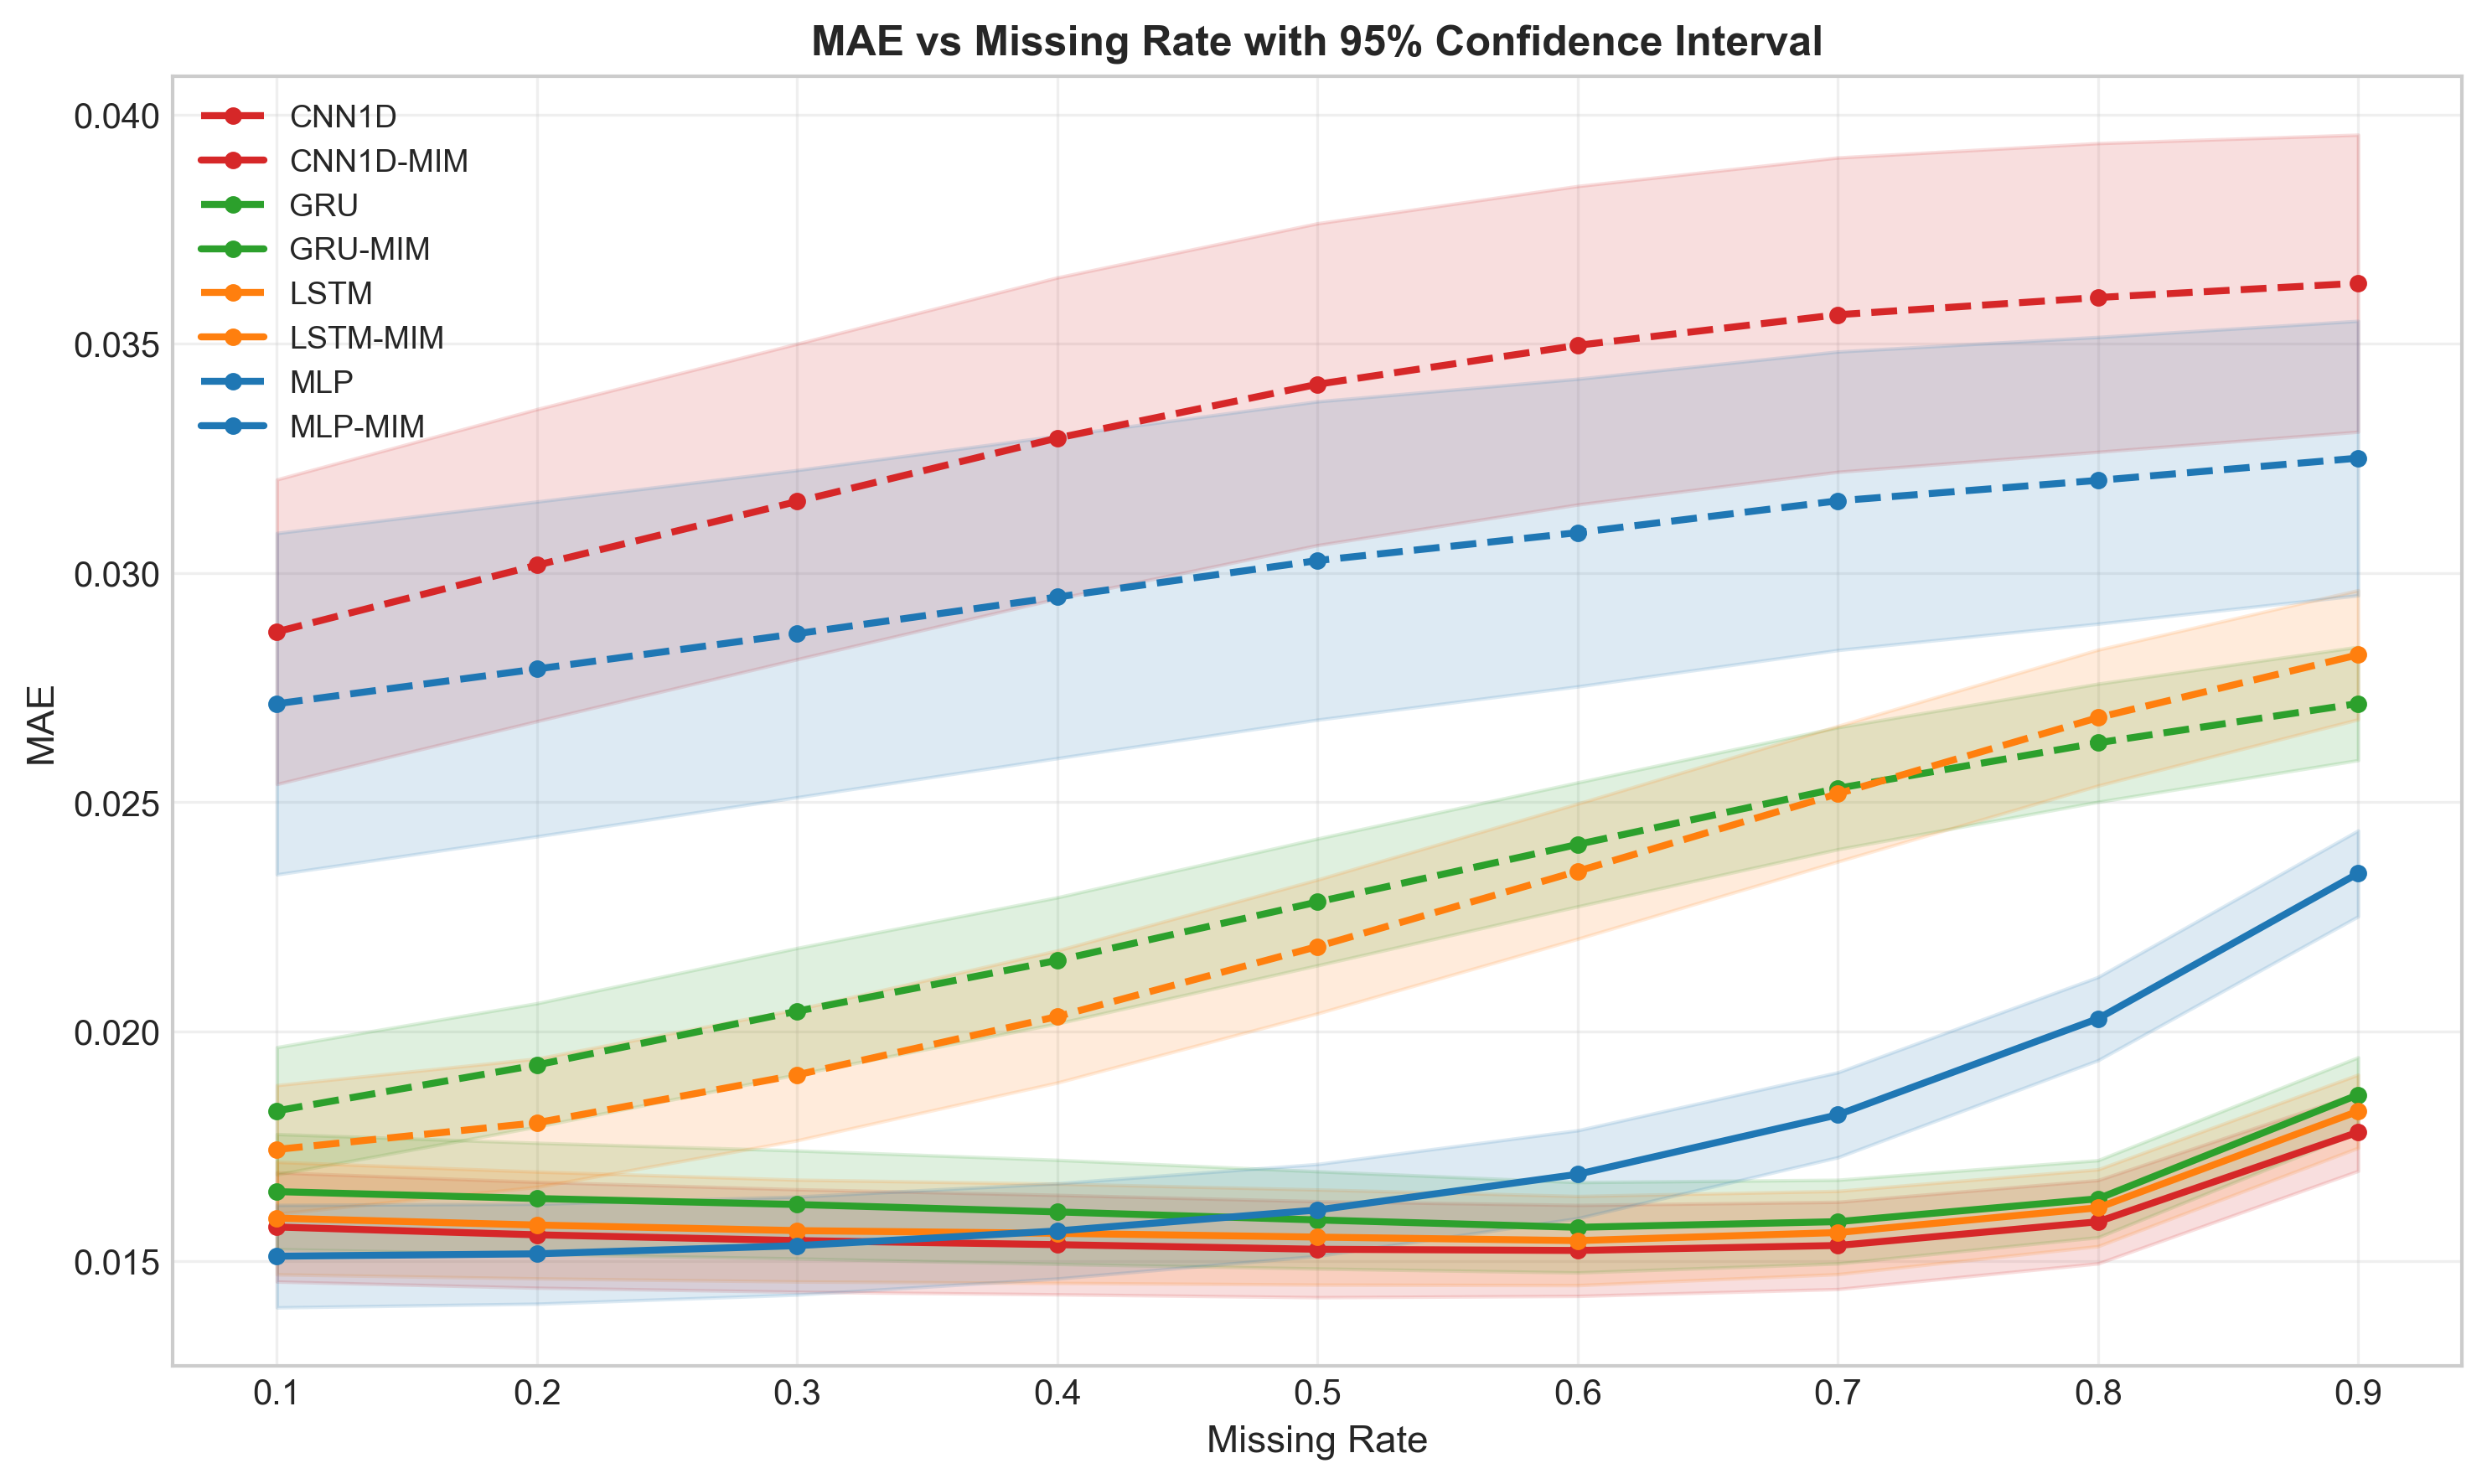
\includegraphics[width=0.48\textwidth]{mae_curves_ci.png}%
        \label{fig:mae_curves}%
    }%
    \hfill
    \subfloat[RMSE curves]{%
        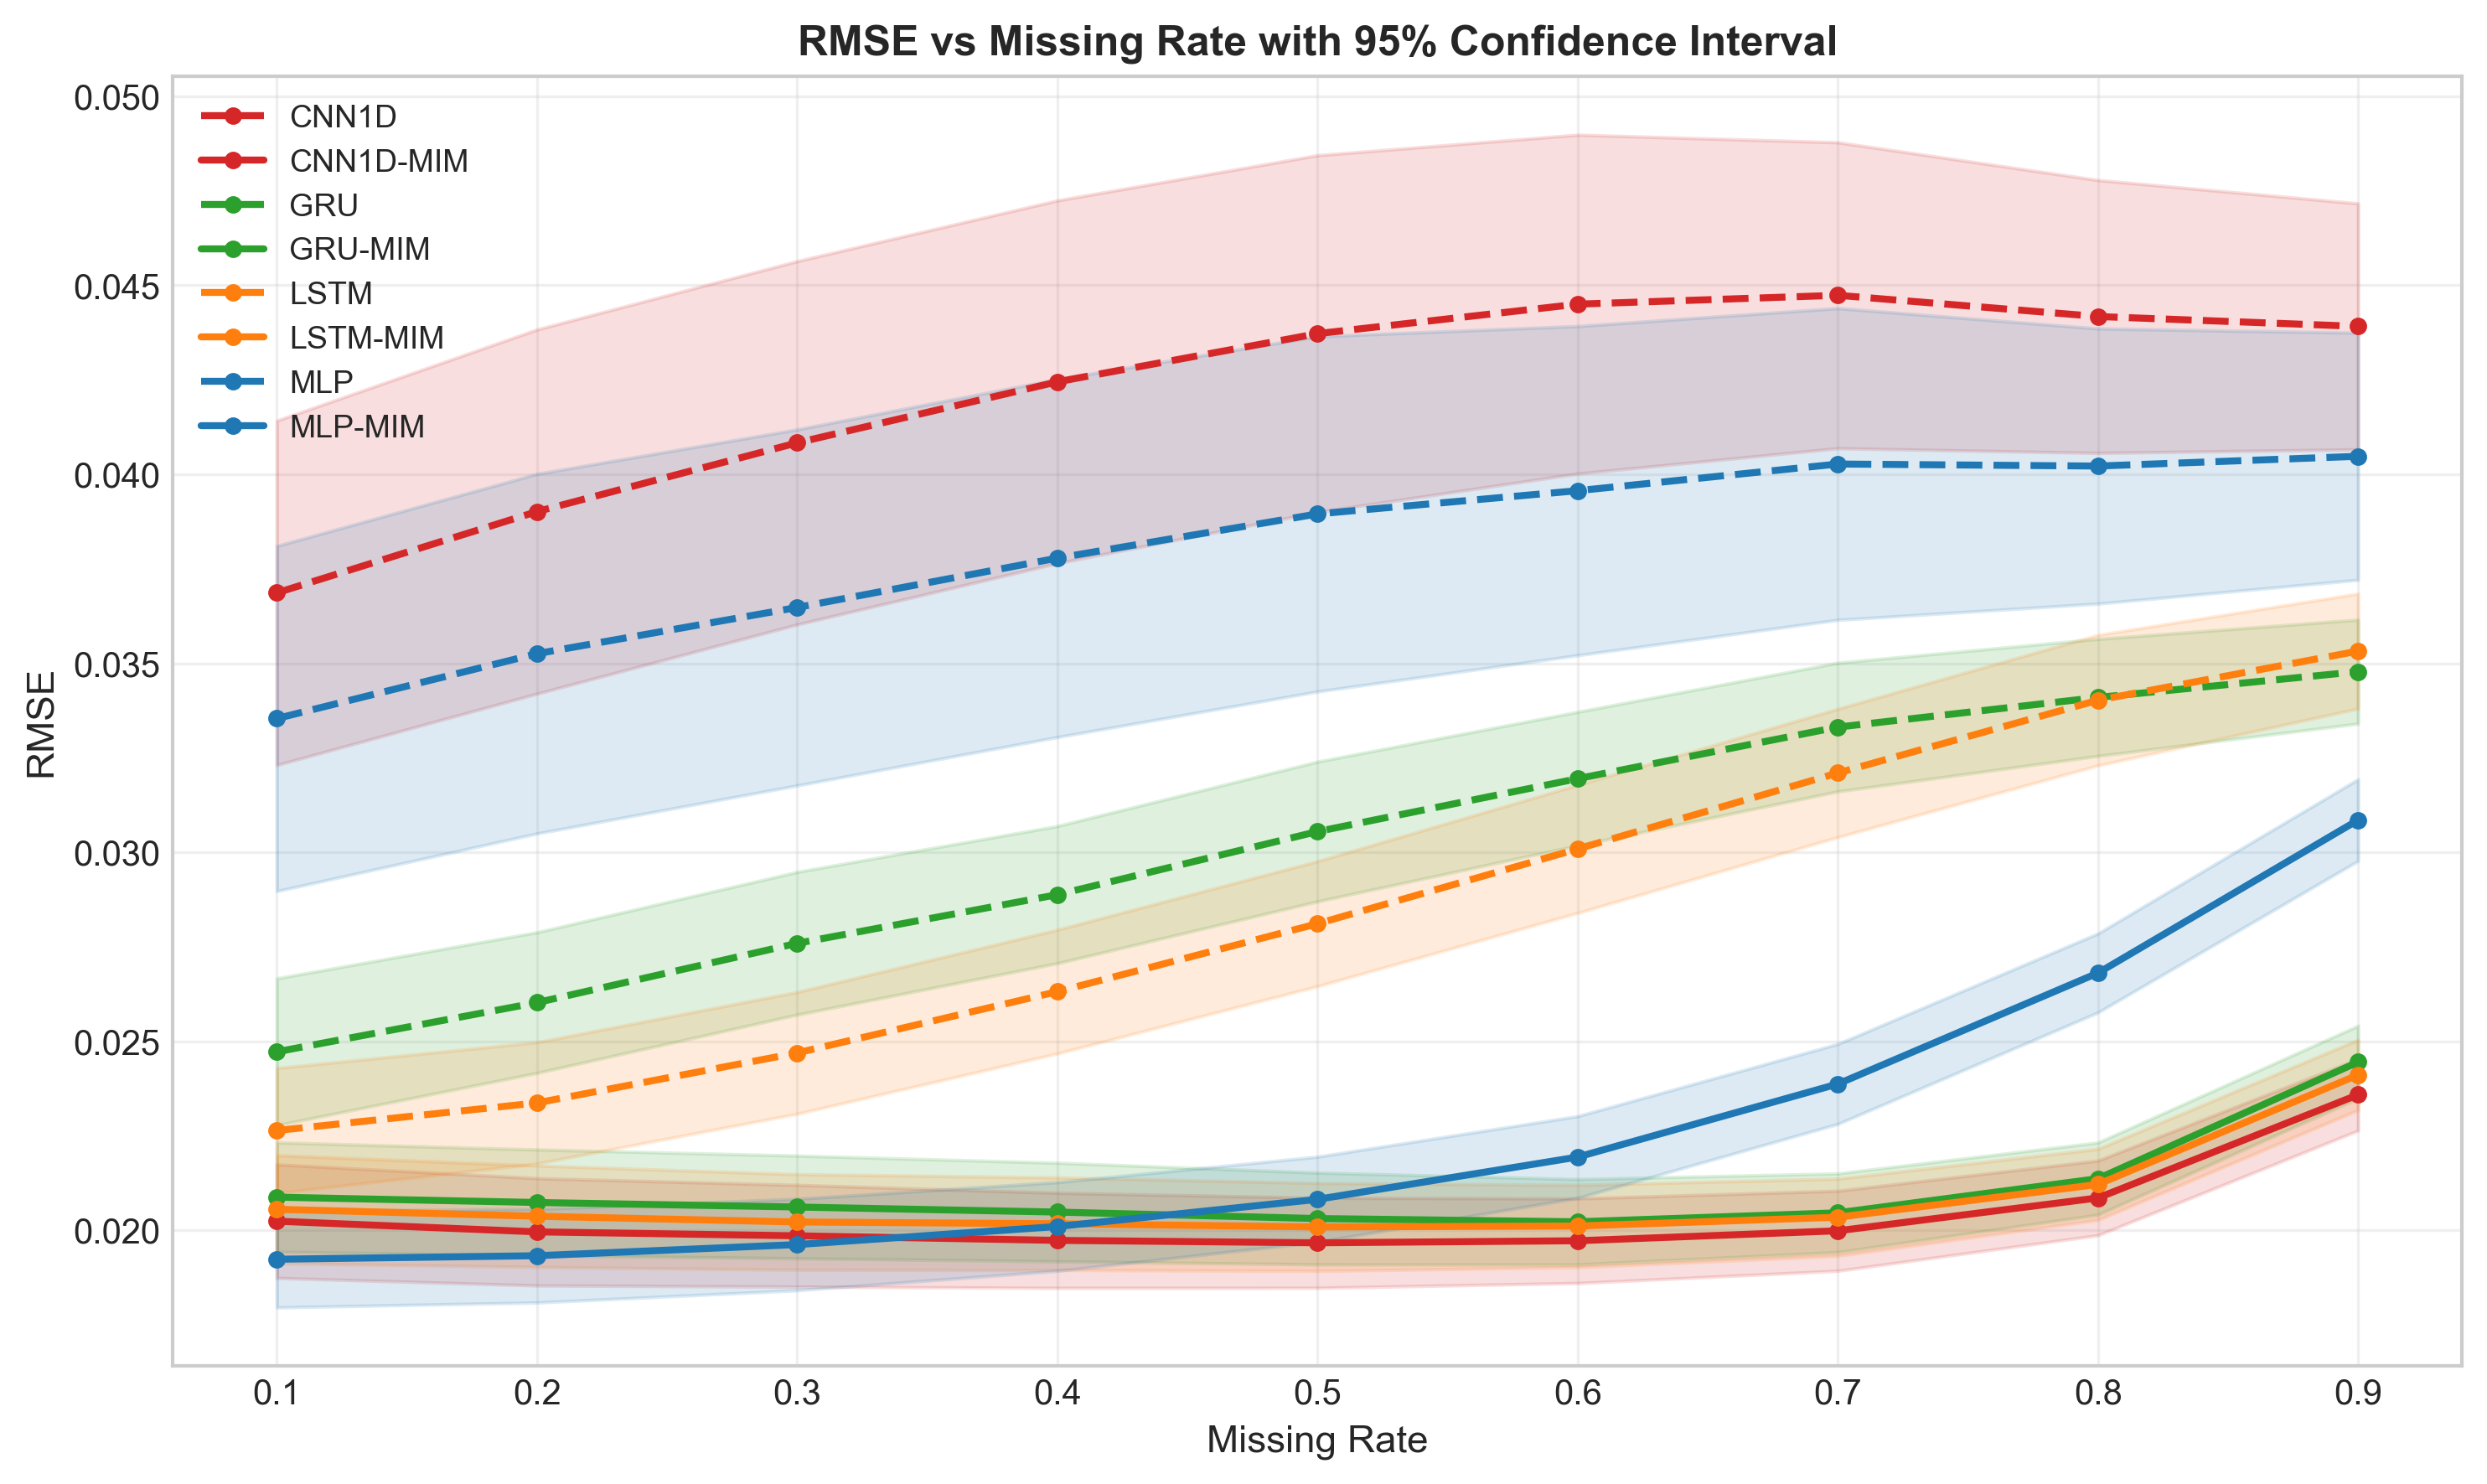
\includegraphics[width=0.48\textwidth]{rmse_curves_ci.png}%
        \label{fig:rmse_curves}%
    }%
    \\
    \subfloat[$R^2$ curves]{%
        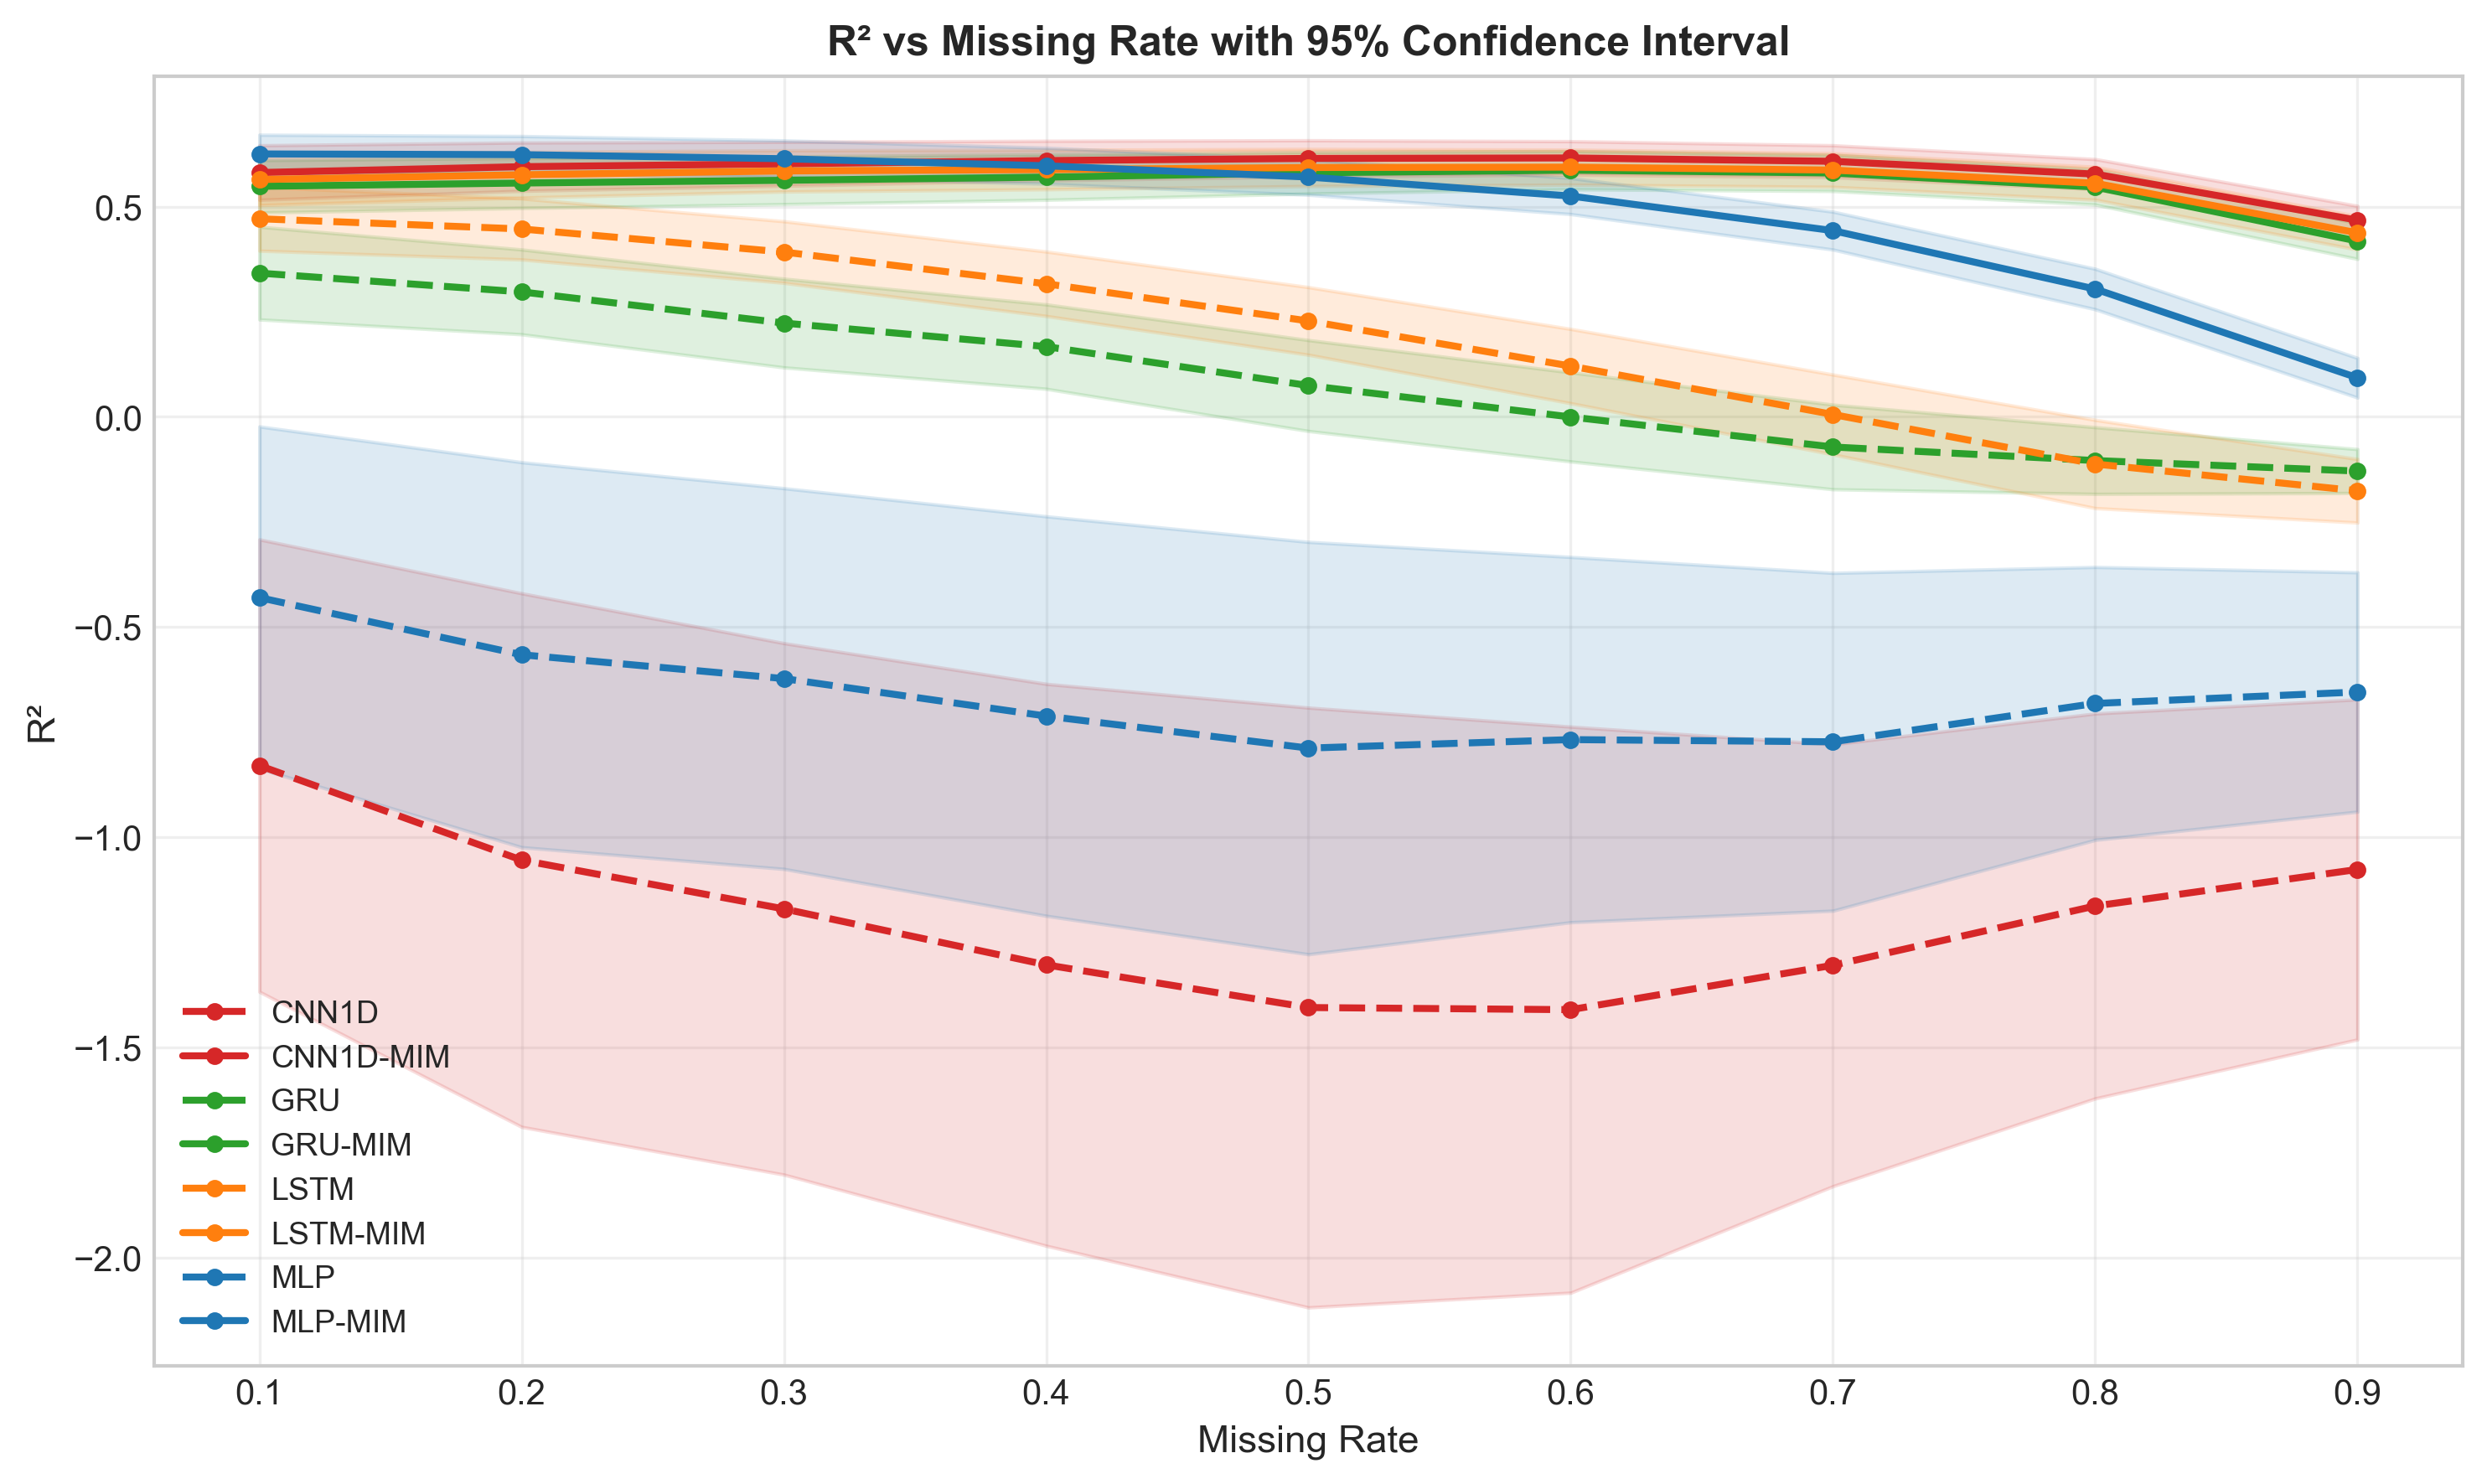
\includegraphics[width=0.48\textwidth]{r2_curves_ci.png}%
        \label{fig:r2_curves}%
    }%
    \hfill
    \subfloat[MAE improvement rates]{%
        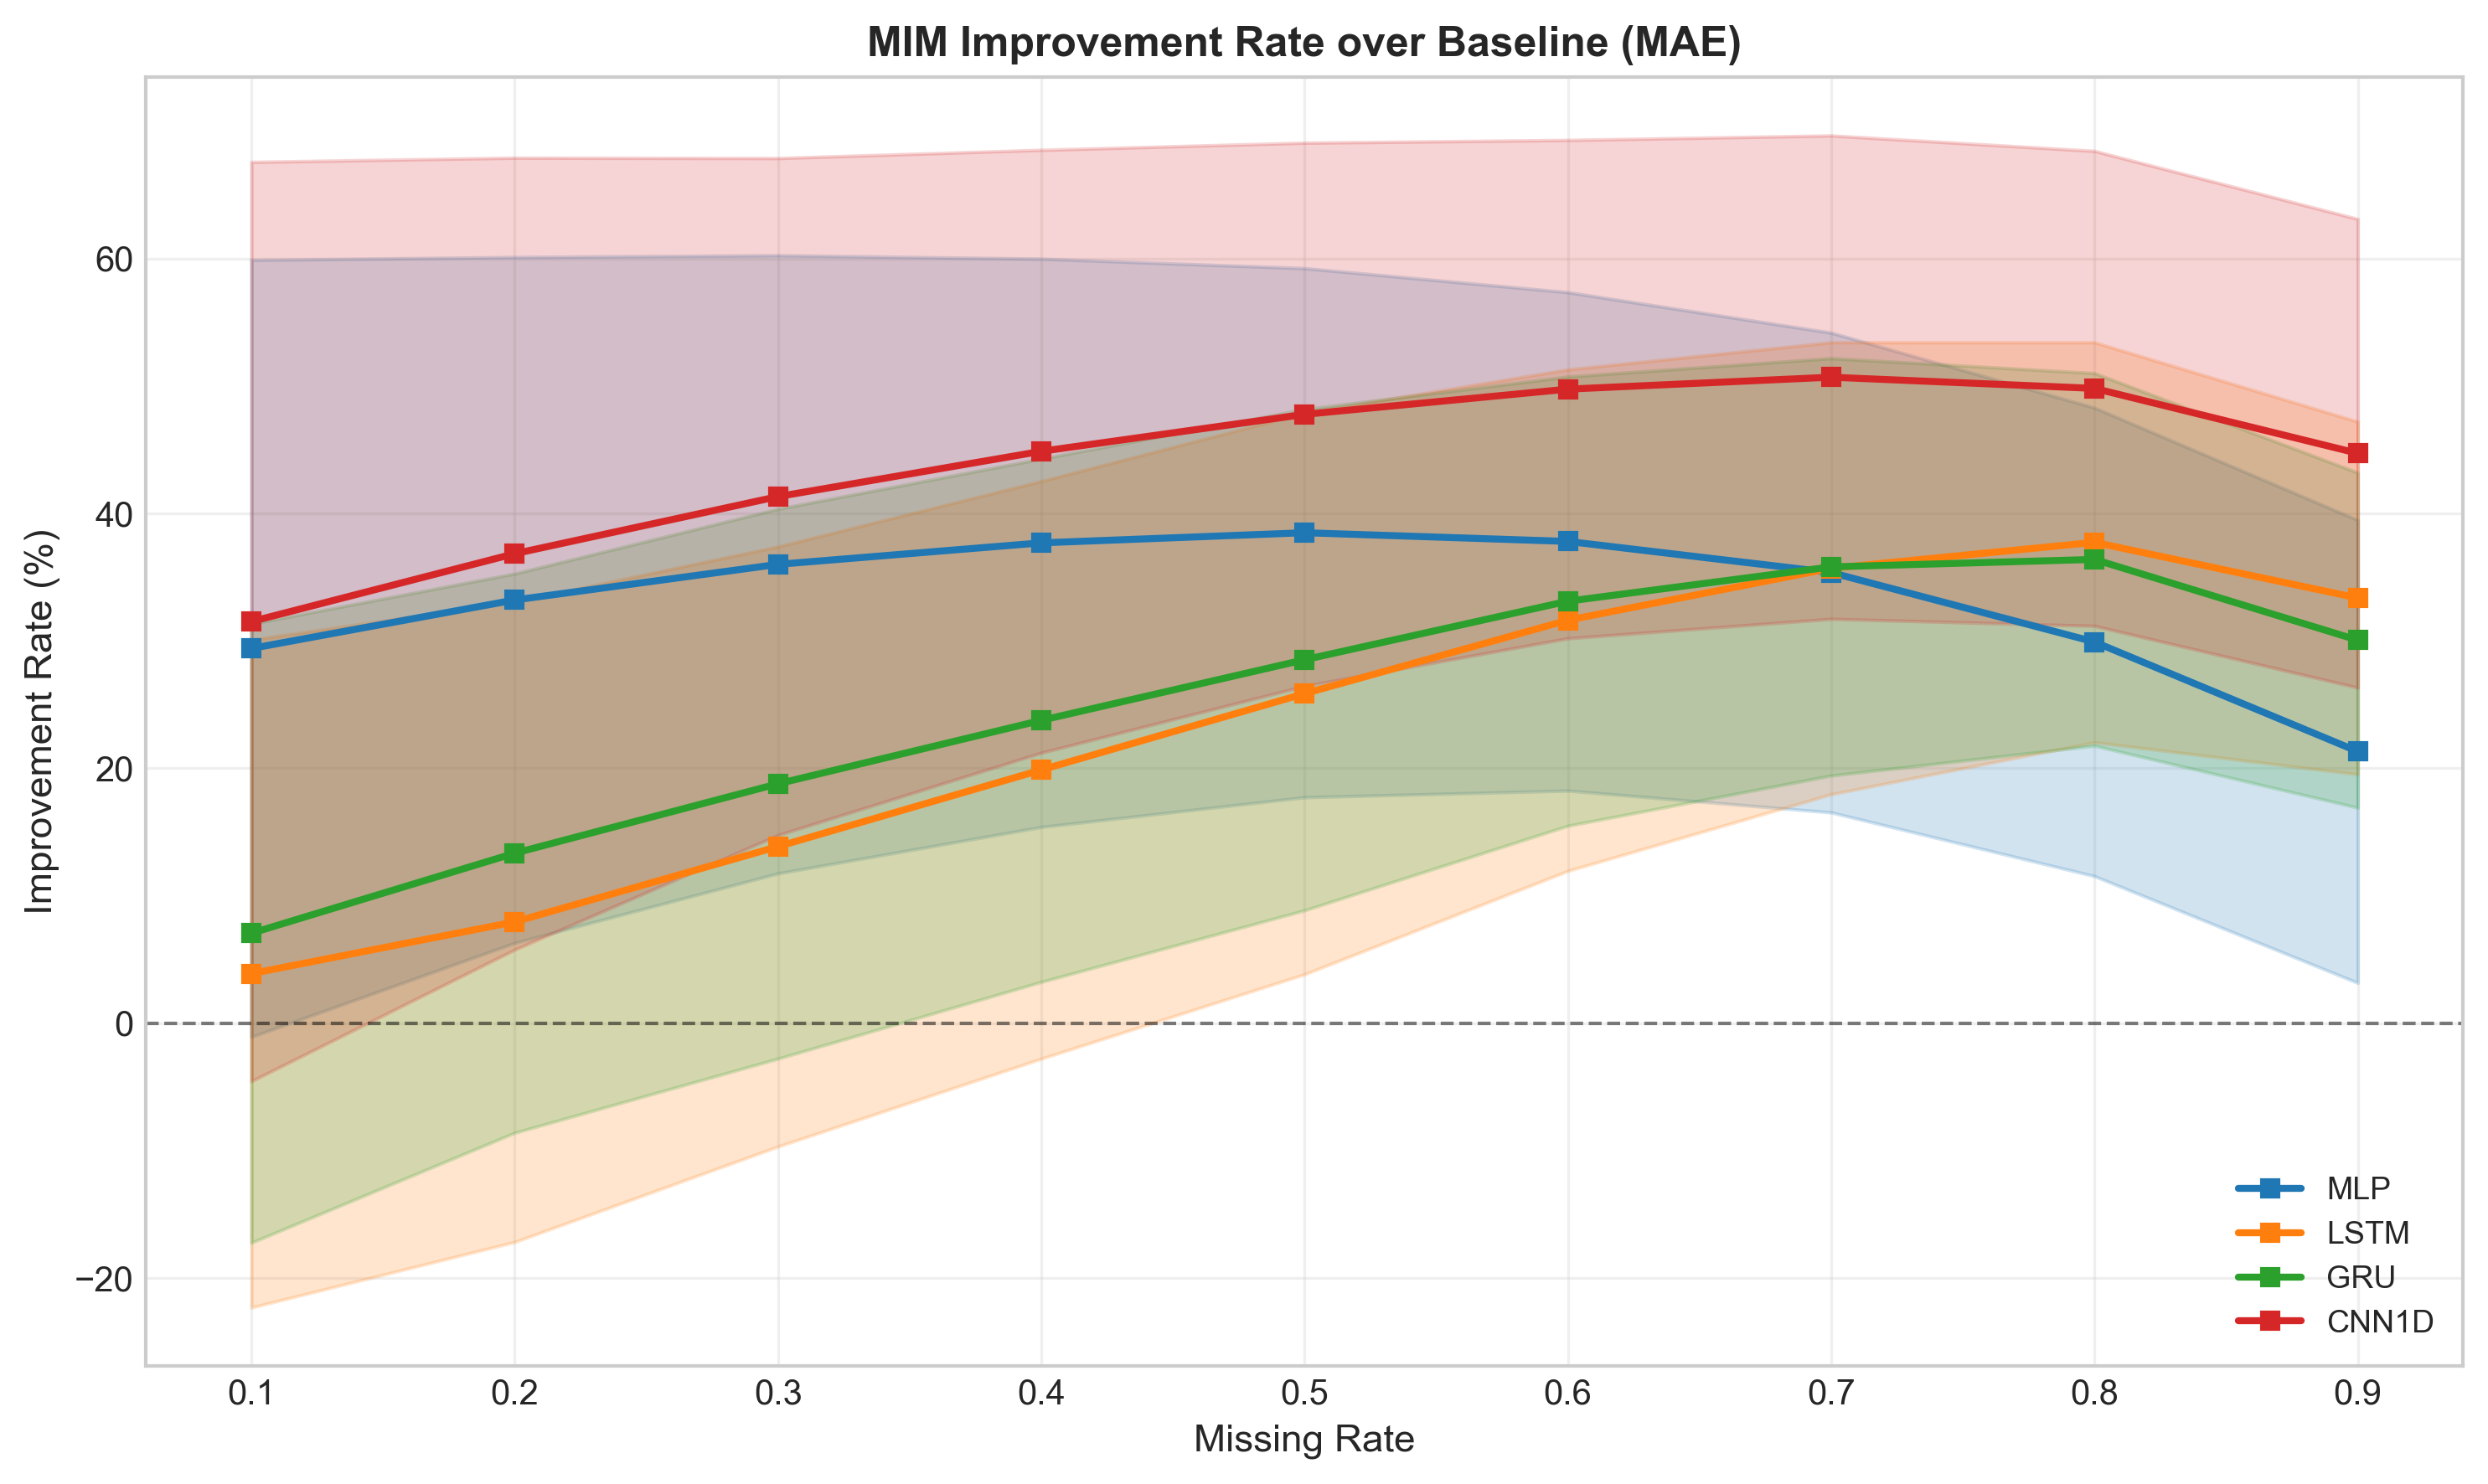
\includegraphics[width=0.48\textwidth]{mae_improvement_rate.png}%
        \label{fig:improvement_rate}%
    }%
    \caption{Comprehensive performance comparison across different metrics and missing rates. (a--c) Metric curves: solid lines for MIM, dashed lines for Baseline, shaded regions for 95\% confidence intervals; (d) Improvement rate curves showing relative error reduction of MIM vs Baseline.}
    \label{fig:performance_metrics}
\end{figure*}

\begin{table*}[!htbp]
\centering
\small
\caption{MAE Comparison and Improvement Rates Under Different Missing Rates (100 random seeds, mean$\pm$std, best values bolded)}
\label{tab:full_results}
\begin{tabular}{@{}llcccc@{}}
\toprule
\textbf{Model} & \textbf{Strategy} & \textbf{MR=0.3} & \textbf{MR=0.5} & \textbf{MR=0.7} & \textbf{MR=0.9} \\
\midrule
\multirow{3}{*}{MLP} 
& Baseline & 0.029$\pm$0.018 & 0.030$\pm$0.017 & 0.032$\pm$0.016 & 0.033$\pm$0.015 \\
& MIM & \textbf{0.015}$\pm$0.005 & \textbf{0.016}$\pm$0.005 & \textbf{0.018}$\pm$0.005 & \textbf{0.023}$\pm$0.005 \\
& Improvement & 46.5\% & 46.8\% & 42.4\% & 27.9\% \\
\midrule
\multirow{3}{*}{LSTM} 
& Baseline & 0.019$\pm$0.007 & 0.022$\pm$0.007 & 0.025$\pm$0.007 & 0.028$\pm$0.007 \\
& MIM & \textbf{0.016}$\pm$0.006 & \textbf{0.016}$\pm$0.005 & \textbf{0.016}$\pm$0.005 & \textbf{0.018}$\pm$0.004 \\
& Improvement & 17.8\% & 29.0\% & 38.0\% & 35.3\% \\
\midrule
\multirow{3}{*}{GRU} 
& Baseline & 0.020$\pm$0.007 & 0.023$\pm$0.007 & 0.025$\pm$0.007 & 0.027$\pm$0.006 \\
& MIM & \textbf{0.016}$\pm$0.006 & \textbf{0.016}$\pm$0.005 & \textbf{0.016}$\pm$0.005 & \textbf{0.019}$\pm$0.004 \\
& Improvement & 20.6\% & 30.4\% & 37.4\% & 31.4\% \\
\midrule
\multirow{3}{*}{1D-CNN} 
& Baseline & 0.032$\pm$0.017 & 0.034$\pm$0.018 & 0.036$\pm$0.017 & 0.036$\pm$0.016 \\
& MIM & \textbf{0.015}$\pm$0.006 & \textbf{0.015}$\pm$0.005 & \textbf{0.015}$\pm$0.005 & \textbf{0.018}$\pm$0.004 \\
& Improvement & 51.1\% & 55.3\% & 57.0\% & 51.0\% \\
\bottomrule
\end{tabular}
\end{table*}

%------------------------------------------------------------------------------
\subsection{Improvement Rates and Statistical Significance}\label{sec:improvement}

The magnitude of MIM's performance benefits is quantified through improvement rate analysis. The improvement rate is defined as:
\begin{equation}
    \text{Improvement}(\%) = \frac{\text{MAE}_{\text{Baseline}} - \text{MAE}_{\text{MIM}}}{\text{MAE}_{\text{Baseline}}} \times 100\%
\end{equation}

Table~\ref{tab:improvement_summary} summarizes improvement rates across all missing rates and architectures. Key observations include:

1D-CNN consistently achieves the highest improvement rates across all missing rates, averaging 52.6\% overall. This suggests that convolutional architectures particularly benefit from the explicit missing pattern information provided by MIM, likely due to their local receptive fields effectively utilizing the spatial structure of missing indicators alongside feature values.

LSTM and GRU exhibit improvement rates that increase monotonically with missing rate (from approximately 18\%/21\% at MR = 0.3 to 38\%/37\% at MR = 0.7), indicating that recurrent architectures become increasingly dependent on missing pattern information as data incompleteness grows. Their gating mechanisms appear to leverage missing indicators to selectively weight reliable versus uncertain inputs.

Wilcoxon signed-rank tests conducted across 100 random seeds confirm that all MIM improvements are statistically significant ($p <$ 0.05), with the vast majority achieving $p <$ 0.001 (Table~\ref{tab:significance}). This robust statistical validation rules out the possibility that observed improvements arise from random variation in initialization or data partitioning.

The improvement rate curves (Figure~\ref{fig:performance_metrics}d) clearly illustrate the architecture-dependent profiles: 1D-CNN maintains consistently high improvement rates (45--57\%) across all missing rates, while LSTM and GRU show monotonically increasing benefits as missing rate rises, crossing the 30\% threshold at MR $\geq$ 0.5.

\begin{table}[!htbp]
\centering
\small
\caption{Summary of MAE Improvement Rates of MIM vs Baseline (\%)}
\label{tab:improvement_summary}
\begin{tabularx}{\columnwidth}{@{}lCCCCCC@{}}
\toprule
\textbf{Model} & \textbf{0.1} & \textbf{0.3} & \textbf{0.5} & \textbf{0.7} & \textbf{0.9} & \textbf{Avg.} \\
\midrule
MLP & 44.4 & 46.5 & 46.8 & 42.4 & 27.9 & 42.5 \\
LSTM & 8.6 & 17.8 & 29.0 & 38.0 & 35.3 & 26.5 \\
GRU & 9.6 & 20.6 & 30.4 & 37.4 & 31.4 & 26.9 \\
1D-CNN & 45.2 & 51.1 & 55.3 & 57.0 & 51.0 & 52.6 \\
\bottomrule
\end{tabularx}
\end{table}

\begin{table}[!htbp]
\centering
\small
\caption{Wilcoxon Signed-Rank Test Results (MIM vs Baseline)}
\label{tab:significance}
\begin{tabularx}{\columnwidth}{@{}lCCCC@{}}
\toprule
\textbf{Model} & \textbf{MR=0.3} & \textbf{MR=0.5} & \textbf{MR=0.7} & \textbf{MR=0.9} \\
\midrule
MLP & $<$0.001*** & $<$0.001*** & $<$0.001*** & 0.001** \\
LSTM & $<$0.001*** & $<$0.001*** & $<$0.001*** & $<$0.001*** \\
GRU & $<$0.001*** & $<$0.001*** & $<$0.001*** & $<$0.001*** \\
1D-CNN & $<$0.001*** & $<$0.001*** & $<$0.001*** & $<$0.001*** \\
\bottomrule
\end{tabularx}
\\[3pt]
\footnotesize Note: *** indicates $p<$0.001, ** indicates $p<$0.01, Wilcoxon signed-rank test, two-tailed, $K=$100 random seeds.
\end{table}

%------------------------------------------------------------------------------
\subsection{Architecture-wise Analysis and Extreme Missing Robustness}\label{sec:architecture}

Different deep learning architectures exhibit distinct behaviors under missing data conditions, providing insights into model selection for practical BMS deployment.

The 1D-CNN architecture demonstrates the most robust performance across all missing rates when combined with MIM. Its local receptive field structure appears particularly well-suited to processing the extended input $[\hat{X} | M]$, allowing convolutional filters to simultaneously capture local feature patterns and their corresponding missing status. At extreme missing rates (MR = 0.9), 1D-CNN-MIM maintains MAE as low as 0.018, representing a 51\% improvement over Baseline.

Recurrent architectures show improvement rates that increase with missing rate, suggesting their gating mechanisms effectively utilize missing indicators to modulate information flow. At MR = 0.9, both LSTM-MIM and GRU-MIM achieve MAE around 0.018--0.019, comparable to 1D-CNN-MIM. This indicates that temporal models can leverage missing pattern information to maintain prediction accuracy even when substantial historical data is unavailable.

While MLP-MIM achieves substantial improvements at low-to-moderate missing rates (average 46\% at MR $\leq$ 0.6), its improvement drops to 27.9\% at MR = 0.9. This suggests that fully-connected architectures, lacking explicit spatial or temporal structure, struggle to fully exploit missing pattern information under extreme data scarcity.

Figure~\ref{fig:distribution} illustrates the distribution characteristics of prediction errors across missing rates. As missing rate increases, Baseline model error distributions broaden and shift toward higher values, indicating increased uncertainty and instability. In contrast, MIM-enabled models maintain concentrated error distributions with stable centers, demonstrating enhanced robustness.

\begin{figure*}[!htb]
    \centering
    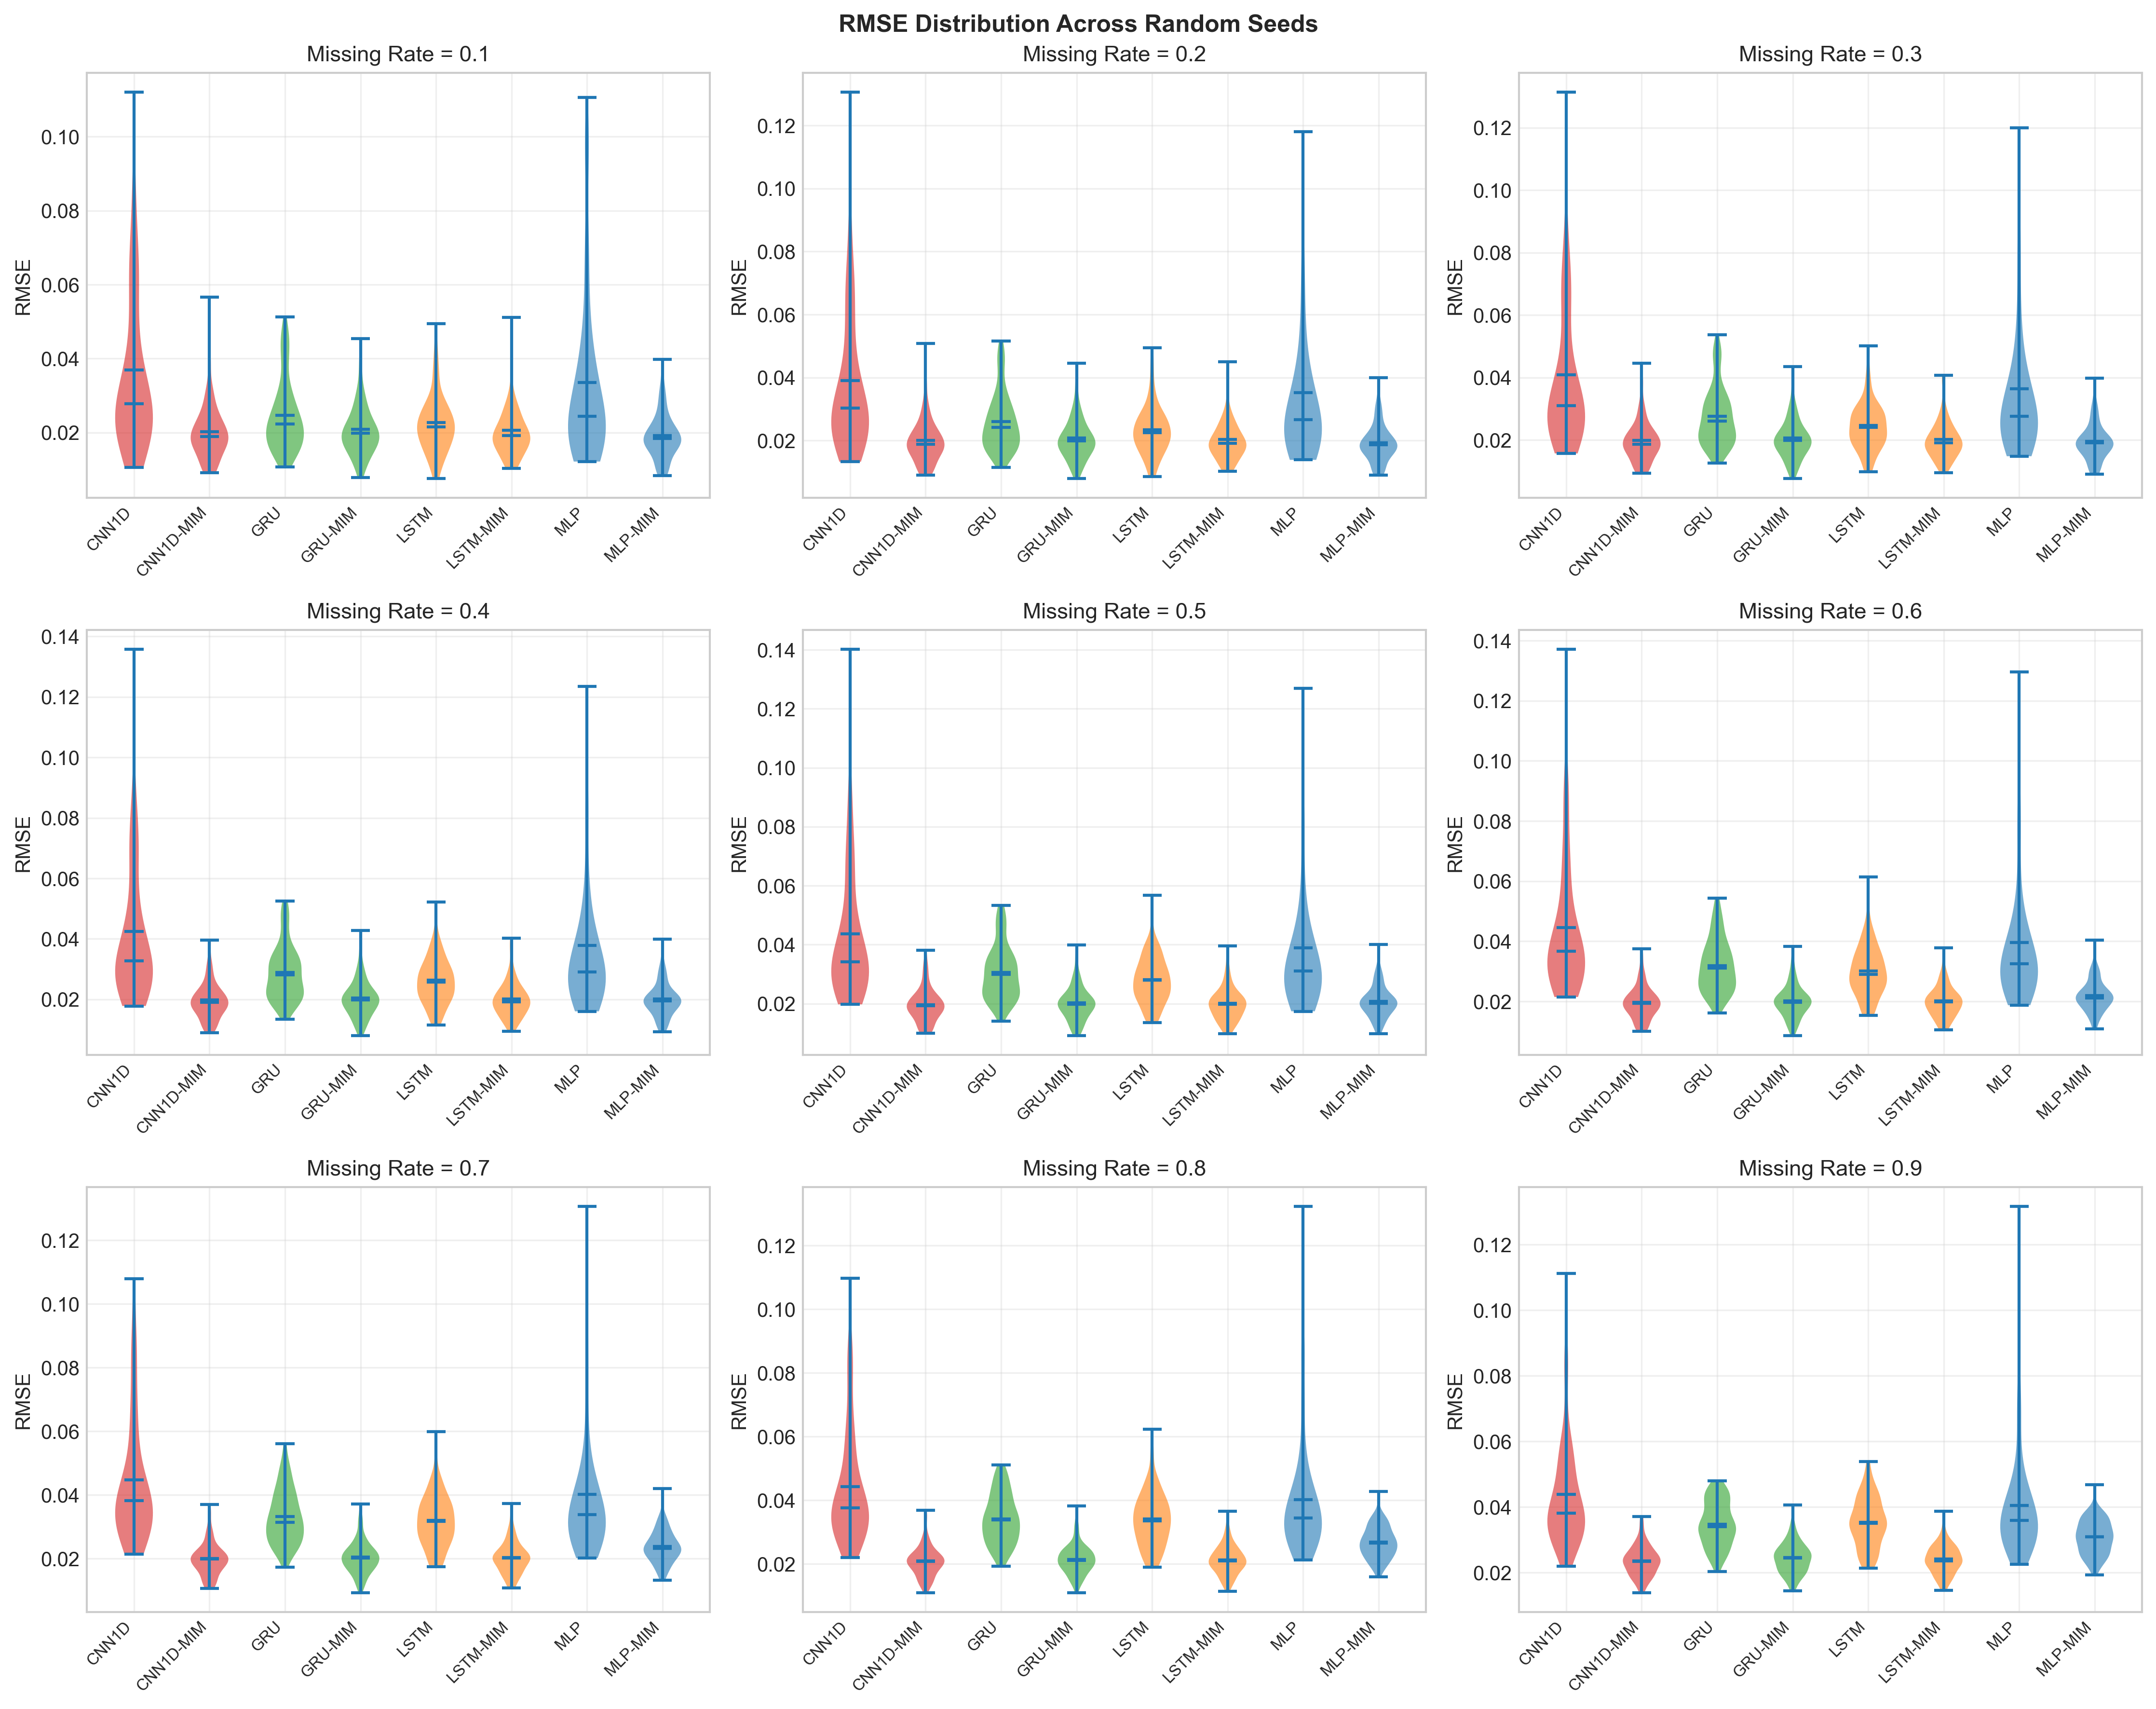
\includegraphics[width=\textwidth]{rmse_distribution.png}
    \caption{MAE distribution under different missing rates (violin plot).}
    \label{fig:distribution}
\end{figure*}

%------------------------------------------------------------------------------
\subsection{Seed Stability and Robustness Analysis}\label{sec:stability}

Beyond average performance, model stability across random initializations is critical for practical deployment. Figure~\ref{fig:seed_stability} presents MAE distributions across 100 independent random seeds.

\begin{figure}[!htbp]
    \centering
    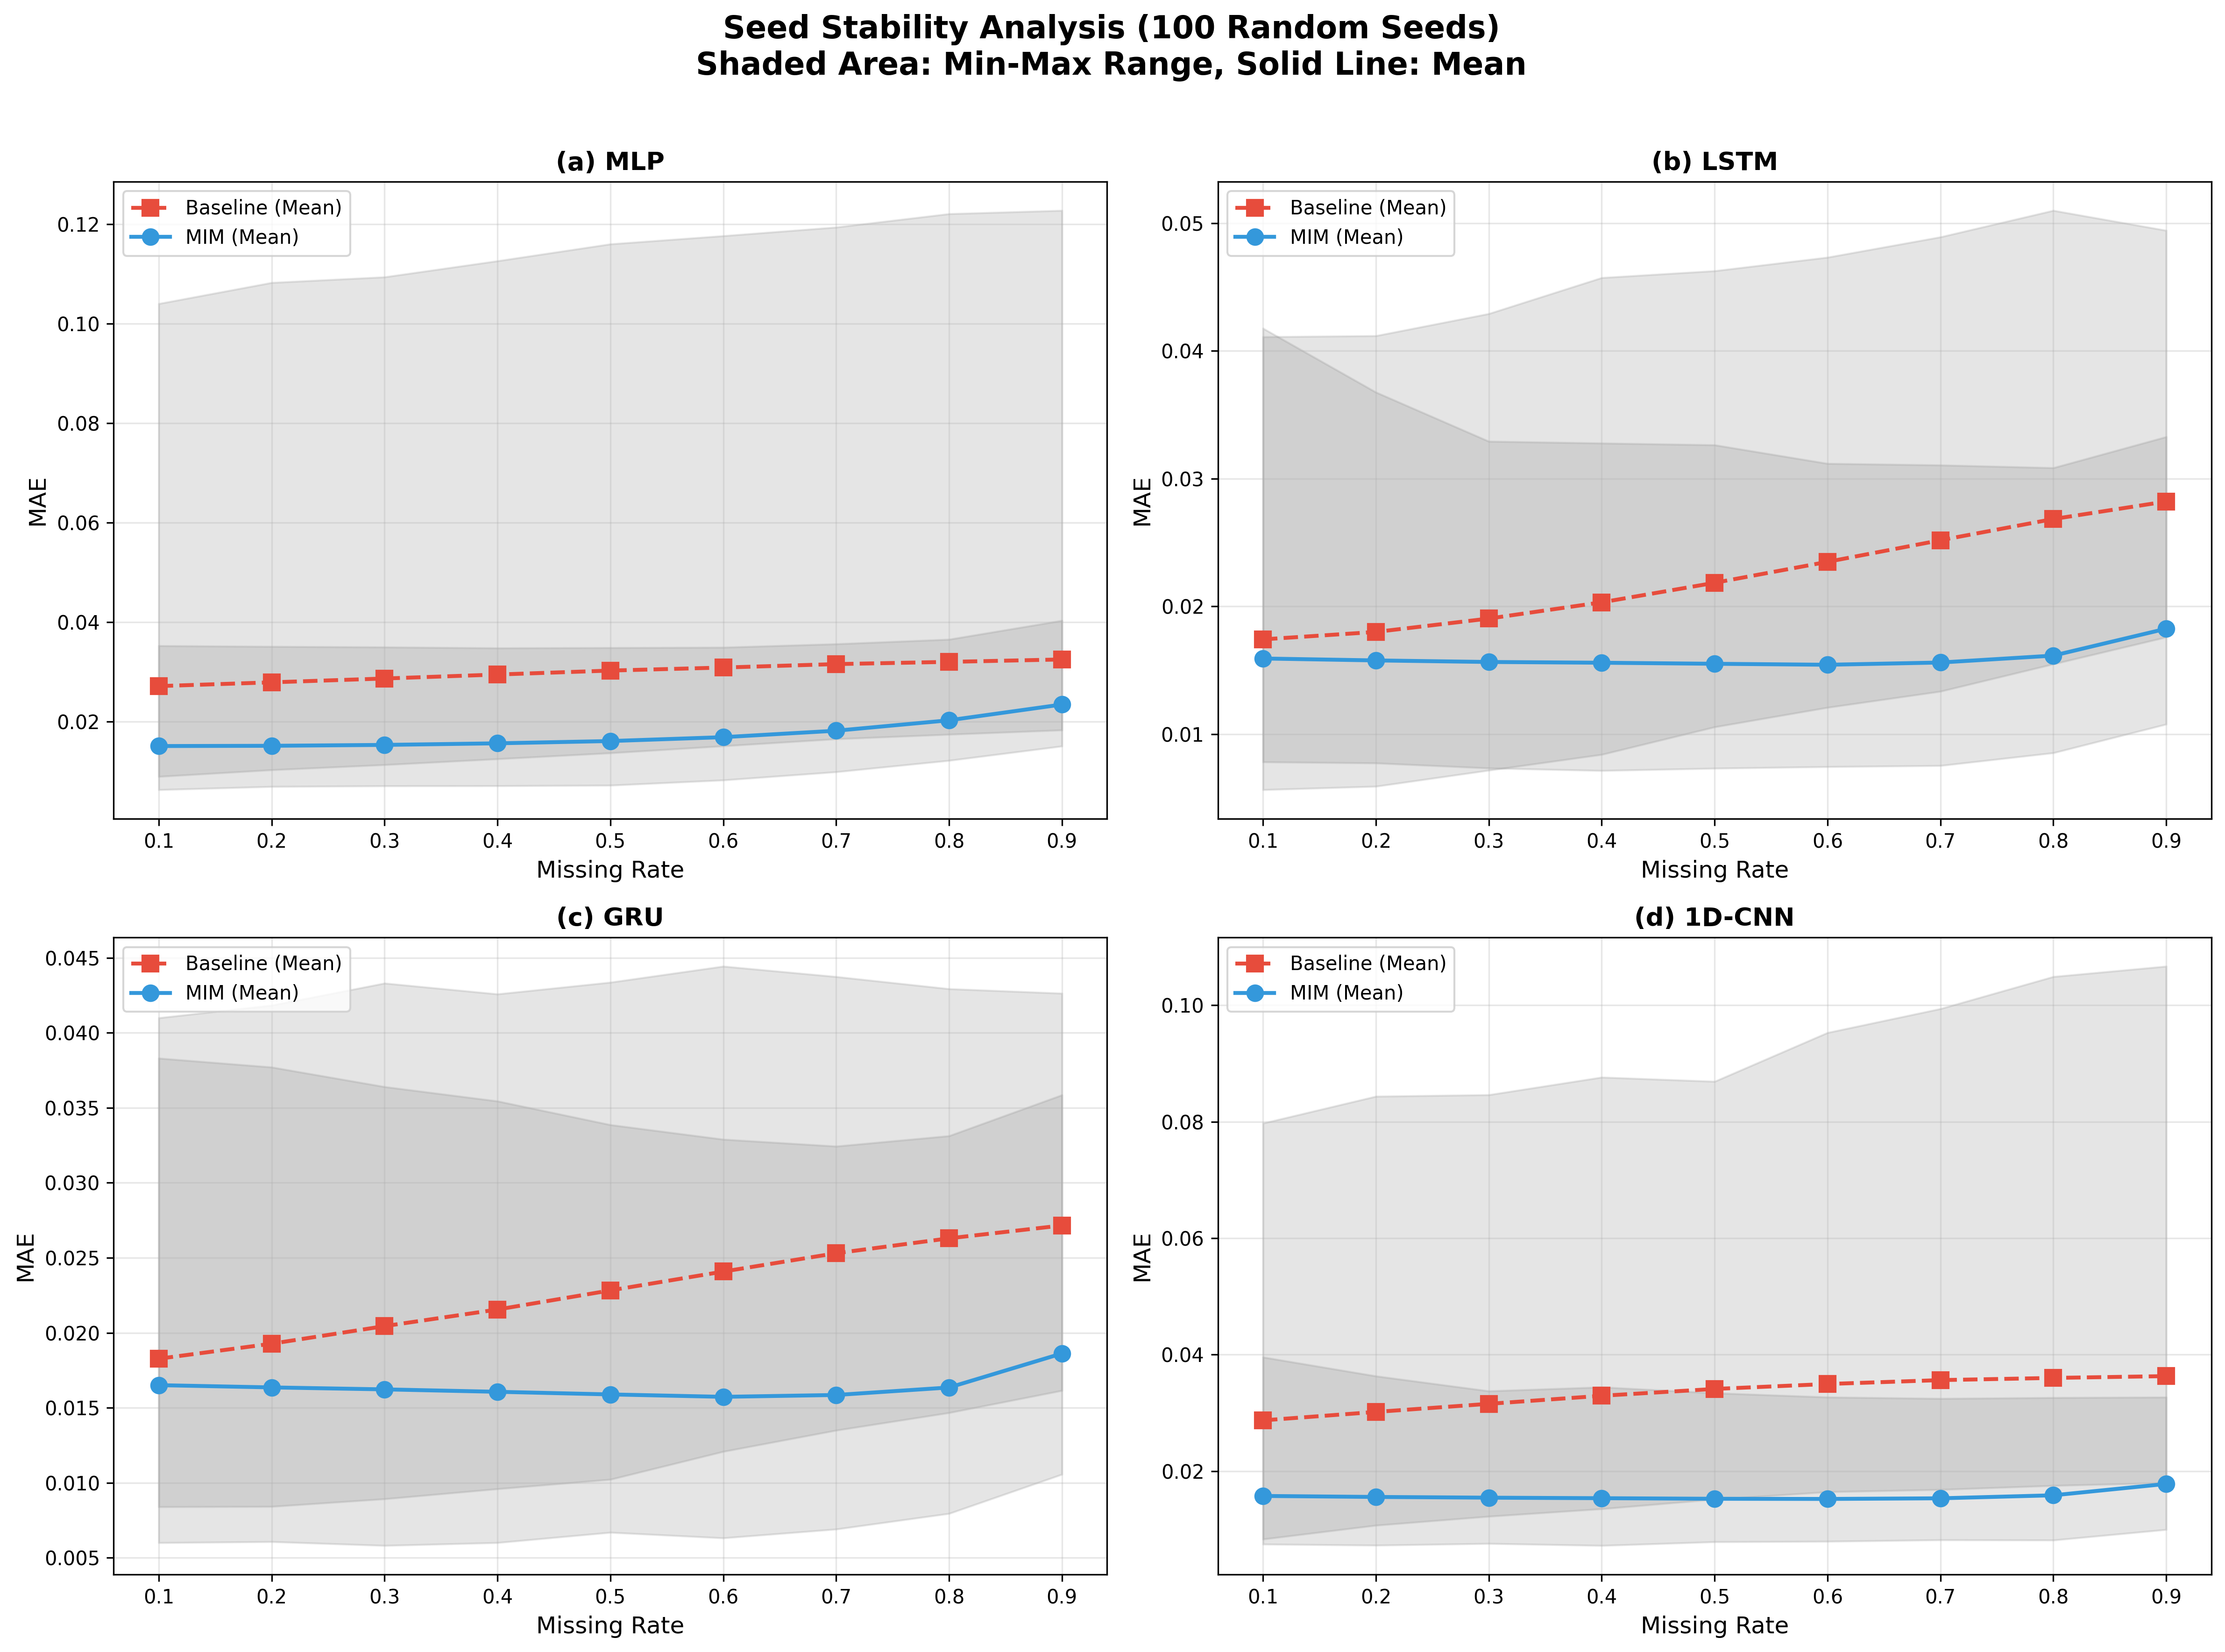
\includegraphics[width=\columnwidth]{fig9_seed_stability_v2.png}
    \caption{Seed stability analysis (100 random seeds). Gray shaded area represents min-max range, colored solid lines represent cross-seed means for MIM, dashed lines represent cross-seed means for Baseline.}
    \label{fig:seed_stability}
\end{figure}

In the medium-to-high missing rate range (MR $\geq$ 0.4), MIM versions exhibit not only lower mean errors but also substantially smaller standard deviations. At MR = 0.5, MIM standard deviations approximate 0.005, compared to Baseline variations of 0.007--0.018. This indicates that MIM significantly reduces model sensitivity to random initialization and data partitioning randomness.

The reduced variance translates to more predictable and reproducible performance in production environments. For BMS applications where consistent behavior across different vehicles or operational periods is essential, MIM's stability advantage represents a significant practical benefit beyond raw accuracy improvements.



%------------------------------------------------------------------------------
\subsection{BMS-Oriented Model and Configuration Recommendations}\label{sec:bms}

Based on the comprehensive experimental results, practical recommendations for BMS deployment under different missing rate scenarios are formulated (Table~\ref{tab:bms_selection}).

In environments with high data quality (MR $\leq$ 0.3), both Baseline and MIM models achieve acceptable performance. For resource-constrained embedded BMS chips, MLP-Baseline provides a computationally efficient solution. If marginal accuracy improvements justify modest additional complexity, MLP-MIM is recommended as the default configuration, offering approximately 44\% error reduction with minimal computational overhead.

As data quality degrades (0.3 $<$ MR $\leq$ 0.6), MIM benefits become substantial. Two configuration options emerge: (1) MLP-MIM as a lightweight efficient solution suitable for edge computing nodes with 46\% improvement at MR = 0.5; (2) 1D-CNN-MIM as a performance-prioritized solution achieving 55\% improvement, appropriate for fleet monitoring systems with adequate computational resources.

Under severe data incompleteness typical of aging sensor networks or harsh operational environments (MR $\geq$ 0.7), MIM becomes essential. 1D-CNN-MIM or LSTM-MIM are recommended, maintaining MAE of 0.018--0.019 even at MR = 0.9. These configurations are suitable for deployment on fleet cloud servers or grid-scale energy storage station controllers where computational resources are less constrained.

\begin{table*}[!htbp]
\centering
\small
\caption{BMS-Oriented Model and MIM Selection Recommendations for Missing Rate Scenarios}
\label{tab:bms_selection}
\begin{tabularx}{\textwidth}{@{}lXX@{}}
\toprule
\textbf{Missing Rate} & \textbf{Recommended Configuration} & \textbf{Engineering Notes} \\
\midrule
MR$\leq$0.3 & MLP-Baseline / MLP-MIM & Low complexity; suitable for embedded BMS chips; MLP-MIM recommended if accuracy margin permits \\
\midrule
0.3$<$MR$\leq$0.6 & MLP-MIM / 1D-CNN-MIM & Medium complexity; edge computing deployment; 46--55\% improvement at MR=0.5 \\
\midrule
MR$\geq$0.7 & 1D-CNN-MIM / LSTM-MIM & Higher complexity; cloud/server deployment; maintains MAE 0.018--0.019 at MR=0.9 \\
\bottomrule
\end{tabularx}
\end{table*}

Regarding computational requirements, MLP-MIM operates with parameter counts on the order of $10^4$, suitable for real-time inference on resource-constrained hardware. 1D-CNN-MIM and LSTM-MIM require moderately higher parameter counts ($2\times10^4$--$4\times10^4$) but remain feasible for modern edge and cloud computing environments. The selection among configurations should consider the trade-off between accuracy requirements, computational budget, and observed missing rate characteristics in the target deployment environment.

Table~\ref{tab:bms_selection} provides a structured decision guide for BMS practitioners, mapping missing rate intervals to recommended model-MIM configurations based on the comprehensive experimental results.



%==============================================================================
\section{Conclusion and Future Work}\label{sec:conclusion}

%------------------------------------------------------------------------------
\subsection{Summary of Findings}\label{sec:findings}

This study systematically investigates the effectiveness of the Missing Indicator Matrix (MIM) approach for battery State of Health prediction under incomplete data conditions. The key findings are summarized as follows:

MIM consistently outperforms traditional imputation-based baselines across the full spectrum of missing rates. The performance advantage is particularly pronounced at moderate-to-high missing rates, where the explicit encoding of missing patterns enables models to maintain prediction accuracy despite substantial information loss. Multi-missing-rate joint training enhances model robustness to unknown missing conditions by exposing models to diverse missing patterns during training, enabling single models to generalize effectively across varying degrees of data incompleteness and mitigating the instability associated with training solely on complete data. Architecture-specific behaviors reveal differential suitability for missing data scenarios, where convolutional and recurrent architectures demonstrate particular advantages in leveraging missing pattern information, maintaining low prediction errors even under extreme missing rates where basic feedforward structures exhibit performance degradation. Finally, cross-seed stability analysis indicates that MIM reduces model sensitivity to random initialization and data partitioning, as incorporating missing indicators not only improves average prediction accuracy but also decreases result variance, enhancing reproducibility and reliability for practical deployment.

%------------------------------------------------------------------------------
\subsection{Practical Implications for BMS Applications}\label{sec:implications}

The findings of this study offer actionable guidance for battery management system design in real-world operational environments:

For deployment scenarios with varying data quality characteristics, the relationship between observed missing rate and optimal model configuration can guide implementation decisions. Low-complexity architectures with MIM suffice for environments with minor data gaps, while more sophisticated models become warranted as missing data prevalence increases.

Rather than treating missing data purely as a preprocessing problem to be eliminated through imputation, BMS designers should consider explicit missing pattern encoding as an integral component of the prediction pipeline. This paradigm shift from ``repair then predict'' to ``predict with awareness'' can substantially enhance system robustness under sensor degradation or communication failures.

The trade-off between model complexity and prediction accuracy varies with missing rate severity. Resource-constrained edge deployments can prioritize lightweight configurations for low-to-moderate missing rates, while cloud-based fleet monitoring systems can leverage more sophisticated architectures to handle severe data incompleteness.

The observed reduction in cross-seed variance with MIM suggests that explicit missing modeling can enhance system reliability across different vehicles, operational periods, and sensor configurations, which is a critical requirement for safety-critical battery health monitoring applications.

%------------------------------------------------------------------------------
\subsection{Limitations and Future Work}\label{sec:future}

This study is limited to the MCAR assumption for controlled experimental conditions; real-world BMS data may exhibit MAR or MNAR patterns where missingness correlates with battery aging. Results are validated on a single dataset with specific battery chemistries, requiring further validation across diverse datasets and operating conditions. Additionally, the evaluation adopts mean imputation as the Baseline and covers four established architectures; future work should explore advanced imputation strategies and emerging model families such as Transformers and physics-informed neural networks.

%==============================================================================
\section*{Acknowledgments}

This work was supported by the Shandong Provincial Technology Innovation Guidance Program (Central Government Guides Local Science and Technology Development Funds) under Grant YDZX2024105.

%==============================================================================
\bibliographystyle{elsarticle-num}
\bibliography{references}

%==============================================================================

\end{document}
